% Options for packages loaded elsewhere
\PassOptionsToPackage{unicode}{hyperref}
\PassOptionsToPackage{hyphens}{url}
%
\documentclass[
  a4paper,
]{book}
\usepackage{amsmath,amssymb}
\usepackage{iftex}
\ifPDFTeX
  \usepackage[T1]{fontenc}
  \usepackage[utf8]{inputenc}
  \usepackage{textcomp} % provide euro and other symbols
\else % if luatex or xetex
  \usepackage{unicode-math} % this also loads fontspec
  \defaultfontfeatures{Scale=MatchLowercase}
  \defaultfontfeatures[\rmfamily]{Ligatures=TeX,Scale=1}
\fi
\usepackage{lmodern}
\ifPDFTeX\else
  % xetex/luatex font selection
\fi
% Use upquote if available, for straight quotes in verbatim environments
\IfFileExists{upquote.sty}{\usepackage{upquote}}{}
\IfFileExists{microtype.sty}{% use microtype if available
  \usepackage[]{microtype}
  \UseMicrotypeSet[protrusion]{basicmath} % disable protrusion for tt fonts
}{}
\makeatletter
\@ifundefined{KOMAClassName}{% if non-KOMA class
  \IfFileExists{parskip.sty}{%
    \usepackage{parskip}
  }{% else
    \setlength{\parindent}{0pt}
    \setlength{\parskip}{6pt plus 2pt minus 1pt}}
}{% if KOMA class
  \KOMAoptions{parskip=half}}
\makeatother
\usepackage{xcolor}
\usepackage{color}
\usepackage{fancyvrb}
\newcommand{\VerbBar}{|}
\newcommand{\VERB}{\Verb[commandchars=\\\{\}]}
\DefineVerbatimEnvironment{Highlighting}{Verbatim}{commandchars=\\\{\}}
% Add ',fontsize=\small' for more characters per line
\usepackage{framed}
\definecolor{shadecolor}{RGB}{248,248,248}
\newenvironment{Shaded}{\begin{snugshade}}{\end{snugshade}}
\newcommand{\AlertTok}[1]{\textcolor[rgb]{0.94,0.16,0.16}{#1}}
\newcommand{\AnnotationTok}[1]{\textcolor[rgb]{0.56,0.35,0.01}{\textbf{\textit{#1}}}}
\newcommand{\AttributeTok}[1]{\textcolor[rgb]{0.13,0.29,0.53}{#1}}
\newcommand{\BaseNTok}[1]{\textcolor[rgb]{0.00,0.00,0.81}{#1}}
\newcommand{\BuiltInTok}[1]{#1}
\newcommand{\CharTok}[1]{\textcolor[rgb]{0.31,0.60,0.02}{#1}}
\newcommand{\CommentTok}[1]{\textcolor[rgb]{0.56,0.35,0.01}{\textit{#1}}}
\newcommand{\CommentVarTok}[1]{\textcolor[rgb]{0.56,0.35,0.01}{\textbf{\textit{#1}}}}
\newcommand{\ConstantTok}[1]{\textcolor[rgb]{0.56,0.35,0.01}{#1}}
\newcommand{\ControlFlowTok}[1]{\textcolor[rgb]{0.13,0.29,0.53}{\textbf{#1}}}
\newcommand{\DataTypeTok}[1]{\textcolor[rgb]{0.13,0.29,0.53}{#1}}
\newcommand{\DecValTok}[1]{\textcolor[rgb]{0.00,0.00,0.81}{#1}}
\newcommand{\DocumentationTok}[1]{\textcolor[rgb]{0.56,0.35,0.01}{\textbf{\textit{#1}}}}
\newcommand{\ErrorTok}[1]{\textcolor[rgb]{0.64,0.00,0.00}{\textbf{#1}}}
\newcommand{\ExtensionTok}[1]{#1}
\newcommand{\FloatTok}[1]{\textcolor[rgb]{0.00,0.00,0.81}{#1}}
\newcommand{\FunctionTok}[1]{\textcolor[rgb]{0.13,0.29,0.53}{\textbf{#1}}}
\newcommand{\ImportTok}[1]{#1}
\newcommand{\InformationTok}[1]{\textcolor[rgb]{0.56,0.35,0.01}{\textbf{\textit{#1}}}}
\newcommand{\KeywordTok}[1]{\textcolor[rgb]{0.13,0.29,0.53}{\textbf{#1}}}
\newcommand{\NormalTok}[1]{#1}
\newcommand{\OperatorTok}[1]{\textcolor[rgb]{0.81,0.36,0.00}{\textbf{#1}}}
\newcommand{\OtherTok}[1]{\textcolor[rgb]{0.56,0.35,0.01}{#1}}
\newcommand{\PreprocessorTok}[1]{\textcolor[rgb]{0.56,0.35,0.01}{\textit{#1}}}
\newcommand{\RegionMarkerTok}[1]{#1}
\newcommand{\SpecialCharTok}[1]{\textcolor[rgb]{0.81,0.36,0.00}{\textbf{#1}}}
\newcommand{\SpecialStringTok}[1]{\textcolor[rgb]{0.31,0.60,0.02}{#1}}
\newcommand{\StringTok}[1]{\textcolor[rgb]{0.31,0.60,0.02}{#1}}
\newcommand{\VariableTok}[1]{\textcolor[rgb]{0.00,0.00,0.00}{#1}}
\newcommand{\VerbatimStringTok}[1]{\textcolor[rgb]{0.31,0.60,0.02}{#1}}
\newcommand{\WarningTok}[1]{\textcolor[rgb]{0.56,0.35,0.01}{\textbf{\textit{#1}}}}
\usepackage{longtable,booktabs,array}
\usepackage{calc} % for calculating minipage widths
% Correct order of tables after \paragraph or \subparagraph
\usepackage{etoolbox}
\makeatletter
\patchcmd\longtable{\par}{\if@noskipsec\mbox{}\fi\par}{}{}
\makeatother
% Allow footnotes in longtable head/foot
\IfFileExists{footnotehyper.sty}{\usepackage{footnotehyper}}{\usepackage{footnote}}
\makesavenoteenv{longtable}
\usepackage{graphicx}
\makeatletter
\def\maxwidth{\ifdim\Gin@nat@width>\linewidth\linewidth\else\Gin@nat@width\fi}
\def\maxheight{\ifdim\Gin@nat@height>\textheight\textheight\else\Gin@nat@height\fi}
\makeatother
% Scale images if necessary, so that they will not overflow the page
% margins by default, and it is still possible to overwrite the defaults
% using explicit options in \includegraphics[width, height, ...]{}
\setkeys{Gin}{width=\maxwidth,height=\maxheight,keepaspectratio}
% Set default figure placement to htbp
\makeatletter
\def\fps@figure{htbp}
\makeatother
\setlength{\emergencystretch}{3em} % prevent overfull lines
\providecommand{\tightlist}{%
  \setlength{\itemsep}{0pt}\setlength{\parskip}{0pt}}
\setcounter{secnumdepth}{5}
\usepackage{booktabs}

\usepackage{titlesec, environ}
\newif\ifcomm\commtrue
\NewEnviron{myanswers}{\ifcomm\BODY\fi}
\ifLuaTeX
  \usepackage{selnolig}  % disable illegal ligatures
\fi
\usepackage[]{natbib}
\bibliographystyle{plainnat}
\IfFileExists{bookmark.sty}{\usepackage{bookmark}}{\usepackage{hyperref}}
\IfFileExists{xurl.sty}{\usepackage{xurl}}{} % add URL line breaks if available
\urlstyle{same}
\hypersetup{
  pdftitle={MATH1710 Probability and Statistics I},
  pdfauthor={Matthew Aldridge},
  hidelinks,
  pdfcreator={LaTeX via pandoc}}

\title{MATH1710 Probability and Statistics I}
\author{\href{https://mpaldridge.github.io/}{Matthew Aldridge}}
\date{University of Leeds, 2023--24}

\usepackage{amsthm}
\newtheorem{theorem}{Theorem}[chapter]
\newtheorem{lemma}{Lemma}[chapter]
\newtheorem{corollary}{Corollary}[chapter]
\newtheorem{proposition}{Proposition}[chapter]
\newtheorem{conjecture}{Conjecture}[chapter]
\theoremstyle{definition}
\newtheorem{definition}{Definition}[chapter]
\theoremstyle{definition}
\newtheorem{example}{Example}[chapter]
\theoremstyle{definition}
\newtheorem{exercise}{Exercise}[chapter]
\theoremstyle{definition}
\newtheorem{hypothesis}{Hypothesis}[chapter]
\theoremstyle{remark}
\newtheorem*{remark}{Remark}
\newtheorem*{solution}{Solution}
\begin{document}
\maketitle

{
\setcounter{tocdepth}{1}
\tableofcontents
}
\hypertarget{schedule}{%
\chapter*{Schedule}\label{schedule}}
\addcontentsline{toc}{chapter}{Schedule}

\newcommand{\Var}{\operatorname{Var}}

\textbf{Week 3} (16--20 October):

\begin{itemize}
\tightlist
\item
  \protect\hyperlink{L05-classical-i}{\textbf{Lecture 5:} Classical probability I} (Monday 16 October)
\item
  \protect\hyperlink{L06-classical-ii}{\textbf{Lecture 6:} Classical probability II} (Wednesday 18 October)
\item
  \textbf{R Practical}
\item
  \protect\hyperlink{P2}{\textbf{Problem Sheet 2:}} Work through in preparation for your tutorial in Week 4. Deadline for assessed questions: Monday 30 October.
\item
  \protect\hyperlink{R}{\textbf{R Worksheet 2:}} Deadline for assessed exercises: Monday 23 October
\item
  \textbf{Office hours:} Friday 20 October, 11--12 and 1--2, \href{boardroom.png}{Maths Boardroom}
\end{itemize}

\textbf{Week 2} (9--13 October):

\begin{itemize}
\tightlist
\item
  \protect\hyperlink{L03-events}{\textbf{Lecture 3:} Sample spaces and events} (Monday 9 October)
\item
  \protect\hyperlink{L04-probability}{\textbf{Lecture 4:} Probability} (Wednesday 11 October)
\item
  \textbf{Tutorial} on \protect\hyperlink{P1}{Problem Sheet 1}
\item
  \protect\hyperlink{practical}{\textbf{R Practical}}
\item
  \protect\hyperlink{P1}{\textbf{Problem Sheet 1:}} Work through in preparation for your tutorial. Deadline for assessed questions: Monday 16 October.
\item
  \protect\hyperlink{R}{\textbf{R Worksheet 1}}
\item
  \textbf{Office hours:} Friday 13 October, 11--12 and 1--2, \href{boardroom.png}{Maths Boardroom}
\end{itemize}

\textbf{Week 1} (2--6 October):

\begin{itemize}
\tightlist
\item
  \protect\hyperlink{L01-stats}{\textbf{Lecture 1:} Summary statistics} (Monday 2 October)
\item
  \protect\hyperlink{L02-dataviz}{\textbf{Lecture 2:} Data visualisation} (Wednesday 4 October)
\item
  \protect\hyperlink{P1}{\textbf{Problem Sheet 1:}} Work through in preparation for your tutorial in Week 2. Deadline for assessed questions: Monday 16 October.
\item
  \textbf{Office hours:} Friday 6 October, 11--12 and 1--2, \href{boardroom.png}{Maths Boardroom}
\end{itemize}

\hypertarget{about}{%
\chapter*{About MATH1710}\label{about}}
\addcontentsline{toc}{chapter}{About MATH1710}

\hypertarget{organisation}{%
\section*{Organisation of MATH1710}\label{organisation}}
\addcontentsline{toc}{section}{Organisation of MATH1710}

This module is \textbf{MATH1710 Probability and Statistics I}. (A small number of second-year scientists are taking this module as the first half of \textbf{MATH2700 Probability and Statistics for Scientists}.)

This module lasts for 11 weeks from 2 October to 15 December 2023. The exam will take place between 15 and 26 January 2024.

The module leader, the lecturer, and the main author of these notes is Dr Matthew Aldridge (you can call me ``Matt'', ``Matthew'', or ``Dr Aldridge'', pronounced ``\emph{old}-ridge'').

\hypertarget{lectures}{%
\subsection*{Lectures}\label{lectures}}
\addcontentsline{toc}{subsection}{Lectures}

The main way you will learn new material for this module is by attending lectures. There are two lectures per week. Because this is a very large class each lecture will be delivered twice:

\begin{itemize}
\tightlist
\item
  \textbf{Mondays} at 1200 or at 1400, in \href{chem-west-map.png}{Chemistry West LT F}
\item
  \textbf{Wednesdays} at 1500 in \href{chem-west-map.png}{Chemistry West LT F} or at 1600 in \href{https://students.leeds.ac.uk/rooms?type=room\&id=100044}{Roger Stevens LT 20}
\end{itemize}

Check your timetable to see which lecture you are assigned to each day (or \href{(chem-west-map.png)}{click this link for a map of how to get to Chemistry West LT F}.

I recommend taking your own notes during the lecture. I will put brief summary notes from the lectures on this website, but will not reflect all the details I say and write during the lectures. Lectures will go through material quite quickly and the material may be quite difficult, so it's likely you'll want to spend time reading through your notes after the lecture.

You are probably reading the web version of the notes. If you want a PDF copy (to read offline or to print out), it can be downloaded via the top ribbon of the page. (Warning: I have not made as much effort to make the PDF as neat and tidy as I have the web version, and there may be formatting errors.) I am very keen to hear about errors in the notes, mathematical, typographical or otherwise. Please \href{mailto:m.aldridge@leeds.ac.uk}{email me} if think you may have found any.

\emph{Attendance at lectures is compulsory.}

\hypertarget{problem-sheets}{%
\subsection*{Problem Sheets}\label{problem-sheets}}
\addcontentsline{toc}{subsection}{Problem Sheets}

There will be 5 problem sheets. Each problem sheet has a number of short and long questions, for you to work on in your own time to help you learn the material, and two assessed questions, which you should submit for marking. The assessed questions on each problem sheet make up 3\% of your mark on this module, for a total of 15\%. Deadlines are 2pm on Mondays, although I'd recommend completing and submitting the work in the previous week.

\begin{longtable}[]{@{}ccc@{}}
\toprule\noalign{}
Problem Sheet & Lectures covered & Deadline for assessed work \\
\midrule\noalign{}
\endhead
\bottomrule\noalign{}
\endlastfoot
1 & 1 and 2 & Monday 16 October (Week 3) \\
2 & 3--6 & Monday 30 October (Week 5) \\
3 & 7--10 & Monday 13 November (Week 7) \\
4 & 11--14 & Monday 27 November (Week 9) \\
5 & 15--18 & Monday 11 December (Week 11) \\
\end{longtable}

An informal Problem Sheet 6 covering material from Lectures 19 and 20 will be available. Lectures 21 and 22 are revision lectures with no new material.

Assessed questions should be submitted in online through the Gradescope platform. Most students choose to hand-write their solutions on paper and then scan and submit on their phone using the Gradescope app. Further Gradescope details to follow nearer the first deadline.

\hypertarget{tutorials}{%
\subsection*{Tutorials}\label{tutorials}}
\addcontentsline{toc}{subsection}{Tutorials}

Tutorials are small groups of about a dozen students. You have been assigned to one of 34 tutorial groups, each with a member of staff as the tutor. Your tutorial group will meet five times, in Weeks 2, 4, 6, 8, and 10; you should check your timetable to see when and where your tutorial group meets.

The tutorials are an interactive session, where the main goal will be to go over your answers to the non-assessed questions on the problems sheets, which you will have worked on in advance of the tutorial. In this smaller group, you will be able to ask detailed questions of your tutor, and have the chance to discuss your answers to the problem sheet. Your tutor may ask you to present some of your work to your fellow students, or may give you the opportunity to work together with others during the tutorial. Your tutor may be willing to give you a hint on the assessed questions if you've made a first attempt but have got stuck. Because of the much smaller groups, the tutorials are the most valuable type of teaching on the module; you should make sure you attend, and you should be well prepared to ensure you make the most of the opportunity.

My recommended approach to problem sheets and tutorials is the following:

\begin{itemize}
\tightlist
\item
  Work through the problem sheet before the tutorial, spending plenty of time on it, and making multiple efforts at questions you get stuck on. I recommend spending \emph{at least 4 hours per problem sheet}. This is a long time, but you shouldn't expect to be able to answer the hardest questions on a problem sheet without making multiple attempts. You don't have to wait until all lectures in a section are complete until starting to work on some of the questions. Collaboration is encouraged when working through the non-assessed problems, but I recommend writing up your work on your own; answers to assessed questions must be solely your own work.
\item
  Take advantage of the small group setting of the tutorial to ask for help or clarification on questions you weren't able to complete.
\item
  After the tutorial, attempt again the questions you were previously stuck on.
\item
  If you're still unable to complete a question after this second round of attempts, \emph{then} consult the solutions.
\end{itemize}

Your tutor will also be the marker of your answers to the assessed questions on the problem sheets.

\emph{Attendance at tutorials is compulsory.}

\hypertarget{r-worksheets}{%
\subsection*{R Worksheets and Practicals}\label{r-worksheets}}
\addcontentsline{toc}{subsection}{R Worksheets and Practicals}

R is a programming language that is particularly good at working with probability and statistics. Learning to use R is an important part of this module, and is used in many other modules in the University, including MATH1712 Probability and Statistics II. R is used by statisticians throughout academia and increasingly in industry too. Learning to program is a valuable skill for all students, and learning to use R is particularly valuable for students interested in statistics and related topics like actuarial science.

You will learn R by working through one R worksheet each week in your own time, starting from Week 2. Even-numbered worksheets will also contain a few questions for assessment, which will be due by 2pm Monday the following week (except the last one). Each of these is worth 3\% of your mark for a total of 15\%. You will submit your answers through a Microsoft Form (details to follow later). I recommend spending one hour per week on the week's R worksheet, plus one extra hour if there are assessed questions that week.

\begin{longtable}[]{@{}
  >{\centering\arraybackslash}p{(\columnwidth - 4\tabcolsep) * \real{0.0923}}
  >{\raggedright\arraybackslash}p{(\columnwidth - 4\tabcolsep) * \real{0.4769}}
  >{\centering\arraybackslash}p{(\columnwidth - 4\tabcolsep) * \real{0.4308}}@{}}
\toprule\noalign{}
\begin{minipage}[b]{\linewidth}\centering
Week
\end{minipage} & \begin{minipage}[b]{\linewidth}\raggedright
Worksheet
\end{minipage} & \begin{minipage}[b]{\linewidth}\centering
Deadline for assessed work
\end{minipage} \\
\midrule\noalign{}
\endhead
\bottomrule\noalign{}
\endlastfoot
2 & 1: R basics & --- \\
3 & 2: Vectors & Monday 23 October (Week 4) \\
4 & 3: Data in R & --- \\
5 & 4: Plots I -- Making plots & Monday 6 November (Week 6) \\
6 & 5: Plots II -- Making plots better & --- \\
7 & 6: Discrete distributions & Monday 20 November (Week 8) \\
8 & 7: Discrete random variables & --- \\
9 & 8: Normal distribution & Monday 4 December (Week 10) \\
10 & 9: Law of large numbers & --- \\
11 & 10: Recap & Thursday 14 December (Week 11) \\
\end{longtable}

~

\textbf{R Practical sessions:} You will be introduced you to R in your first Practical session, in Week 2. You will first see how to use R on University computers (these sessions will take place in computer ``clusters''). There will then be an opportunity to install R on your own device -- if you have a laptop on which you want to install R, bring it along to the practical session. A second practical, in Week 3, will allow you to get help on the R Worksheet 2, which is the first worksheet with assessed questions.

There are 11 R practical session groups -- check your timetable for Weeks 2 and 3 to see when and where your group meets.

\emph{Attendance at the first R practical session (Week 2) is compulsory.}

\hypertarget{dropin}{%
\subsection*{``Office hours'' drop-in sessions}\label{dropin}}
\addcontentsline{toc}{subsection}{``Office hours'' drop-in sessions}

If you there is something in the module you wish to discuss one-on-one with the module leader, the place for the is the optional weekly ``office hours'', which will operate as drop-in sessions. These sessions are an optional opportunity for you to ask questions you have to me; these are particularly useful if there's something on the module that you are stuck on or confused about, but I'm happy to discuss any statistics-related issues or questions you have.

I currently plan two ``office hours'' drop-in sessions per week:

\begin{itemize}
\tightlist
\item
  Fridays 1100--1200 and 1300--1400 in the \href{boardroom.png}{Mathematics Boardroom (map)}.
\end{itemize}

I may change arrangements as term continues -- if attendance levels are low, I will move office hours to be actual office.

If neither time is possible, you may \href{mailto:m.aldridge@leeds.ac.uk}{email me} to arrange an alternative time to talk to me.

\emph{Attendance at ``office hours'' sessions is optional.}

\hypertarget{time}{%
\subsection*{Time management}\label{time}}
\addcontentsline{toc}{subsection}{Time management}

It is, of course, up to you how you choose to spend your time on this module. But my recommendations for your work would be something like this:

\begin{itemize}
\tightlist
\item
  \textbf{Lectures:} 2 hours per week, plus 1 hour per week reading through notes.
\item
  \textbf{Problem sheets:} 4 hours per problem sheet, plus 1 extra hour for writing up and submitting answers to assessed questions.
\item
  \textbf{R worksheets:} 1 hour per week, plus 1 extra hour if there are assessed questions.
\item
  \textbf{Tutorials:} 1 hour every other week.
\item
  \textbf{Revision:} 16 hours total at the end of the module.
\item
  \textbf{Exam:} 2 hours.
\end{itemize}

That makes about 100 hours in total. (MATH1710 is a 10-credit module, so is supposed to represent 100 hours work. MATH2700 students are expected to be able to use their greater experience to get through the material in just 75 hours, so should scale these recommendations accordingly.)

\hypertarget{exam}{%
\subsection*{Exam}\label{exam}}
\addcontentsline{toc}{subsection}{Exam}

There will be an exam in January, which makes up the remaining 70\% of your mark. The exam will consist of 20 short and 2 long questions, and will be time-limited to 2 hours. We'll talk more about the exam format near the end of the module.

\hypertarget{ask}{%
\subsection*{Who should I ask about\ldots?}\label{ask}}
\addcontentsline{toc}{subsection}{Who should I ask about\ldots?}

There are over 440 students registered for this module. If each student emails me once a week, and if each email takes me 10 minutes to read and respond, that will take more than 15 hours of my time every day! Generally, it's much better to come to speak to me at the ``office hours'' drop-in session or, if it will be very quick, before or after a lecture.

\begin{itemize}
\tightlist
\item
  \emph{I don't understand something in the notes or on a problem sheet}: Come to office hours, or ask your tutor in your next tutorial.
\item
  \emph{I'm having difficulties with R:} In Weeks 2 or 3, you should ask at your R practical session; at other times, come to office hours.
\item
  \emph{I have an admin question about arrangements for the module:} Come to office hours or talk to me before/after lectures.
\item
  \emph{I have an admin question about arrangements for my tutorial:} Contact your tutor.
\item
  \emph{I have an admin question about general arrangements for my programme as a whole:} \href{https://students.leeds.ac.uk/askingforhelp}{Contact the Student Information Service} or speak to your personal tutor.
\item
  \emph{I have a question about the marking of my assessed work on the Problem Sheets:} First, check your feedback on Gradescope; if you still have questions, contact your tutor.
\item
  \emph{I have a question about the marking of my assessed work on the R Worksheets:} You can \href{mailto:m.aldridge@leeds.ac.uk}{email me} about this.
\item
  \emph{Due to truly exceptional and unforeseeable personal circumstances I require an extension on or exemption from assessed work:} You can apply by \href{https://students.leeds.ac.uk/info/10111/assessment/860/mitigating_circumstances}{filling in the mitigating circumstances form at this link}. Neither I nor your tutor can unilaterally offer an extension or exemption, so please don't ask. (Extensions of up to 4 days are available for Problem Sheets. Only exemptions are available for R Worksheets.)
\end{itemize}

\hypertarget{about-content}{%
\section*{Content of MATH1710}\label{about-content}}
\addcontentsline{toc}{section}{Content of MATH1710}

\hypertarget{prereqs}{%
\subsection*{Prerequisites}\label{prereqs}}
\addcontentsline{toc}{subsection}{Prerequisites}

The formal prerequisite for MATH1710 is ``Grade B in A-level Mathematics or equivalent''. I'll assume you have some basic school-level maths knowledge, but I won't assume you've studied probability or statistics in detail before (although I recognise that many of you will have). If you have studied probability and/or statistics at A-level (or post-16 equivalent) level, you'll recognise some of the material in this module; however you should find that we go deeper in many areas, and that we treat the material through with a greater deal of mathematical formality and rigour. ``Rigour'' here means precisely stating our assumptions, and carefully \emph{proving} how other statements follow from those assumptions.

\hypertarget{syllabus}{%
\subsection*{Syllabus}\label{syllabus}}
\addcontentsline{toc}{subsection}{Syllabus}

The module has three parts: a short first part on ``exploratory data analysis'', a long middle part on probability theory, and a short final part on a statistical framework called ``Bayesian statistics''. There's also the weekly R worksheets, which you could count as a fourth part running in parallel, but which will connect with the other parts too.

An outline plan of the topics covered is the following.

\begin{itemize}
\tightlist
\item
  \textbf{Exploratory data analysis} {[}2 lectures{]}: Summary statistics, data visualisation
\item
  \textbf{Probability} {[}16 lectures{]}:

  \begin{itemize}
  \tightlist
  \item
    Probability with events: Probability spaces, probability axioms, examples and properties of probability, ``classical probability'' of equally likely events, independence, conditional probability, Bayes' theorem {[}6 lectures{]}
  \item
    Probability with random variables: Discrete random variables, expectation and variance, binomial distribution, geometric distribution, Poisson distribution, multiple random variables, law of large numbers, continuous random variables, exponential distribution, normal distribution, central limit theorem {[}10 lectures{]}
  \end{itemize}
\item
  \textbf{Bayesian statistics} {[}2 lectures{]}: Bayesian framework, Beta prior, normal--normal model
\item
  Summary and revision {[}2 lectures{]}
\end{itemize}

You'll notice that this module is heavier on the ``Probability'' than the ``Statistics'' of its title. MATH1712 Probability and Statistics II, on the other hand, which many students on this module will take next semester, is almost entirely ``Statistics'', but uses probabilistic techniques developed here.

\hypertarget{books}{%
\subsection*{Books}\label{books}}
\addcontentsline{toc}{subsection}{Books}

You can do well on this module by attending the lectures and tutorials, and working on the problem sheets and R worksheets, without needing to do any further reading beyond this. However, students can benefit from optional pre-reading in advance, extra background reading, or an alternative view on the material, especially in the parts of the module on probability. These books are also a good place to look if you want extra exercises and problems for revision.

For exploratory data analysis, you can stick to Wikipedia, but if you really want a book, I'd recommend:

\begin{itemize}
\tightlist
\item
  GM Clarke and D Cooke, \emph{A Basic Course in Statistics}, 5th edition, Edward Arnold, 2004.
\end{itemize}

For the probability section, any book with a title like ``Introduction to Probability'' would do. Some of my favourites are:

\begin{itemize}
\tightlist
\item
  JK Blitzstein and J Hwang, \emph{Introduction to Probability}, 2nd edition, CRC Press, 2019.
\item
  G Grimmett and D Welsh, \emph{Probability: An Introduction}, 2nd edition, Oxford University Press, 2014. (The library has \href{https://leeds.primo.exlibrisgroup.com/permalink/44LEE_INST/13rlbcs/alma991002938669705181}{online access}.)
\item
  SM Ross, \emph{A First Course in Probability}, 10th edition, Pearson, 2020.
\item
  RL Scheaffer and LJ Young, \emph{Introduction to Probability and Its Applications}, 3rd edition, Cengage, 2010.
\item
  D Stirzaker, \emph{Elementary Probability}, 2nd edition, Cambridge University Press, 2003. (The library has \href{https://leeds.primo.exlibrisgroup.com/permalink/44LEE_INST/13rlbcs/alma991013131349705181}{online access}.)
\end{itemize}

I also found lecture notes by \href{https://people.maths.bris.ac.uk/~maotj/teaching.html}{Prof Oliver Johnson} (University of Bristol) and \href{http://www.statslab.cam.ac.uk/~rrw1/prob/index.html}{Prof Richard Weber} (University of Cambridge) to be useful.

On Bayesian statistics, we will only taste a brief introduction, but if you want a book, I recommend:

\begin{itemize}
\tightlist
\item
  JV Stone, \emph{Bayes' Rule: A Tutorial Introduction to Bayesian Analysis}, Sebtel Press, 2013.
\end{itemize}

For R, there are many excellent resources online.

(For all these books I've listed the newest editions, but older editions are usually fine too.)

\hypertarget{about-notes}{%
\section*{About these notes}\label{about-notes}}
\addcontentsline{toc}{section}{About these notes}

These notes were written by Matthew Aldridge in 2021, and were edited and updated a lot in 2022 and a little bit in 2023. They are based in part on previous notes by Dr Robert G Aykroyd and Prof Wally Gilks. Dr Jason Susanna Anquandah and Dr Aykroyd advised on the R worksheets. Dr Aykroyd's help and advice on many aspects of the module was particularly valuable.

These notes (in the web format) should be accessible by screenreaders. If you have accessibility difficulties with these notes, \href{mailto:m.aldridge@leeds.ac.uk}{contact me}.

\hypertarget{part-part-i-exploratory-data-analysis}{%
\part*{Part I: Exploratory data analysis}\label{part-part-i-exploratory-data-analysis}}
\addcontentsline{toc}{part}{Part I: Exploratory data analysis}

\hypertarget{L01-stats}{%
\chapter{Summary statistics}\label{L01-stats}}

\hypertarget{what-is-eda}{%
\section{What is EDA?}\label{what-is-eda}}

\textbf{Statistics} is the study of data. \textbf{Exploratory data analysis} (or \textbf{EDA}, for short) is the part of statistics concerned with taking a ``first look'' at some data. Later, toward the end of this module, we will see more detailed and complex ways of building models for data, and in MATH1712 Probability and Statistics II (for those who take it) you will see many other statistical techniques -- in particular, ways of testing formal hypotheses for data. But here we're just interested in first impressions and brief summaries.

In this section, we will concentrate on two aspects of EDA:

\begin{itemize}
\tightlist
\item
  \textbf{Summary statistics:} That is, calculating numbers that briefly summarise the data. A summary statistic might tell us what ``central'' or ``typical'' values of the data are, how spread out the data is, or about the relationship between two different variables.
\item
  \textbf{Data visualisation:} Drawing a picture based on the data is an another way to show the shape (centrality and spread) of data, or the relationship between different variables.
\end{itemize}

Even before calculating summary statistics or drawing a plot, however, there are other questions it is important to ask about the data:

\begin{itemize}
\tightlist
\item
  \emph{What is the data?} What variables have been measured? How were they measured? How many datapoints are there? What is the possible range of responses?
\item
  \emph{How was the data collected?} Was data collected on the whole population or just a smaller sample? If a sample: How was that sample chosen? Is that sample representative of the population?
\item
  \emph{Are there any outliers?} ``Outliers'' are datapoints that seem to be very different from the other datapoints -- for example, are much larger or much smaller than the others. Each outlier should be investigated to seek the reason for it. Perhaps it is a genuine-but-unusual datapoint (which is useful for understanding the extremes of the data), or perhaps there is an extraordinary explanation (a measurement or recording error, for example) meaning the data is not relevant. Once the reason for an outlier is understood, it then \emph{might} be appropriate to exclude it from analysis (for example, the incorrectly recorded measurement). It's usually bad practice to exclude an outlier merely for being an outlier before understanding what caused it.
\item
  \emph{Ethical questions:} Was the data collected ethically and, where necessary, with the informed consent of the subjects? Has it been stored properly? Are their privacy issues with the collection and storage of the data? What ethical issues should be considered before publishing (or not publishing) results of the analysis? Should the data be kept confidential, or should it be openly shared with other researchers for the betterment of science?
\end{itemize}

\hypertarget{what-is-R}{%
\section{What is R?}\label{what-is-R}}

\textbf{R} is a programming language that is particularly good at working with probability and statistics. A convenient way to use the language R is through the program \textbf{RStudio}. An important part of this module is learning to use R, by completing weekly worksheets -- you can read more in \protect\hyperlink{R}{the R section of these notes}.

R can easily and quickly perform all the calculations and draw all the plots in this section of notes on exploratory data analysis. In this text, we'll show the relevant R code. Code will appear like this:

\begin{Shaded}
\begin{Highlighting}[]
\NormalTok{data }\OtherTok{\textless{}{-}} \FunctionTok{c}\NormalTok{(}\DecValTok{4}\NormalTok{, }\DecValTok{7}\NormalTok{, }\DecValTok{6}\NormalTok{, }\DecValTok{7}\NormalTok{, }\DecValTok{4}\NormalTok{, }\DecValTok{5}\NormalTok{, }\DecValTok{5}\NormalTok{)}
\FunctionTok{mean}\NormalTok{(data)}
\end{Highlighting}
\end{Shaded}

\begin{verbatim}
[1] 5.428571
\end{verbatim}

Here, the code in the first shaded box is the R commands that are typed into
RStudio, which you can type in next to the \texttt{\textgreater{}} arrow in the RStudio ``console''. The numerical answers that R returns are shown here in the second unshaded box. The \texttt{{[}1{]}} can be ignored (this is just R's way of saying that this is the first part of the answer -- but the answer here only has one part anyway). Plots produced by R are displayed in these notes as pictures.

Most importantly for now, \emph{you are not expected to understand the R code in this section yet}. The code is included so that, in the future, as you work through the R worksheets week by week, you can look back at the code in the section, and it will start to make sense. By the time you have finished R Worksheet 5 in Week 6, you should be able understand most of the R code in this section.

\hypertarget{stat-central}{%
\section{Statistics of centrality}\label{stat-central}}

Suppose we have collected some data on a certain variable. We will assume here that we have \(n\) datapoints, each of which is a single real number. We can write this data as a vector
\[ \mathbf x = (x_1, x_2, \dots, x_n) . \]

A \textbf{statistic} is a calculation from the data \(\mathbf x\), which is (usually) also a real number. In this section we will look at two types of ``summary statistics'', which are statistics that we feel will give us useful information about the data.

We'll look here at two types of summary statistic:

\begin{itemize}
\tightlist
\item
  \textbf{Statistics of centrality}, which tell us where the ``middle'' of the data is.
\item
  \textbf{Statistics of spread}, which tell us how far the data typically spreads out from that middle.
\end{itemize}

Some measures of centrality are the following.

\begin{definition}

Consider some real-valued data \(\mathbf x = (x_1, x_2, \dots, x_n)\).

\begin{itemize}
\tightlist
\item
  The \textbf{mode} is the most common value of \(x_i\). (If there are multiple joint-most common values, they are all modes.)
\item
  Suppose the data is ordered as \(x_1 \leq x_2 \leq \cdots \leq x_n\). Then the \textbf{median} is the central value in the ordered list. If \(n\) is odd, this is \(x_{(n+1)/2}\); if \(n\) is even, we normally take halfway between the two central points, \(\frac12(x_{n/2}+x_{n/2 + 1})\).
\item
  The \textbf{mean} \(\bar x\) is
  \[ \bar x = \frac{1}{n}(x_1 + x_2 + \cdots + x_n) = \frac1n \sum_{i=1}^n x_i . \]
\end{itemize}

\end{definition}

In that last expression, we've made use of Sigma notation to write down the sum. (If Sigma notation is new to you, I recommend \href{https://www.mathcentre.ac.uk/resources/workbooks/mathcentre/sigma.pdf}{this PDF from MathCentre}, or Section 2.4 of Clarke and Cooke, \emph{A Basic Course in Statistics}.)

\begin{example}
Some packets of Skittles (a small fruit-flavoured sweet) were opened, and the number of Skittles in each packet counted. There were 13 packets, and the number of sweets (sorted from smallest to largest) were:
\[ 59, \ 59, \ 59, \ 59, \ 60, \ 60, \ 60, \ 61, \ 62, \ 62, \ 62, \ 63, \ 63 .\]

The mode is 59, because there were 4 packets containing 59 sweets; more than any other number.

Since there are \(n = 13\) packets, the middle packet is number \(i = 7\), so the median is \(x_7 = 60\).

The mean is
\[ \bar x = \frac{1}{13} (59 + 59 + \cdots + 63) = \frac{789}{13} = 60.7 .\]
\end{example}

The median is one example of a ``quantile'' of the data. Suppose our data is increasing order again. For \(0 \leq \alpha \leq 1\), the \textbf{\(\alpha\)-quantile} \(q(\alpha)\) of the data is the datapoint \(\alpha\) of the way along the list. Generally, \(q(\alpha)\) is equal to \(x_{1+\alpha(n-1)}\) when \(1+\alpha(n-1)\) is an integer. (If \(1+\alpha(n-1)\) isn't an integer, there are various conventions of how to choose that we won't go into here. R has \emph{nine} different settings for choosing quantiles! -- we will always just use R's default choice.)

\begin{itemize}
\tightlist
\item
  The \textbf{median} is the \(\frac12\)-quantile \(q(\frac12)\), which is \(q(\frac12) = x_7 = 60\) for this data.
\item
  The \textbf{minimum} is the 0-quantile \(q(0)\), which is \(q(0) = x_1 = 59\) for this data.
\item
  The \textbf{maximum} is the 1-quantile \(q(1)\), which is \(q(1) = x_{13} = 63\) for this data
\item
  The \textbf{lower quartile} (that's ``quartile'', as in ``quarter'' -- not ``quantile'') is the \(\frac14\)-quantile \(q(\frac14)\), which is \(q(\frac14) = x_4 = 59\) for this data.
\item
  The \textbf{upper quartile} is the \(\frac34\)-quantile \(q(\frac34)\), which is \(q(\frac34) = x_{10} = 62\) for this data.
\end{itemize}

The following R code reads in some data which has the daily average temperature in Leeds in 2020, divided into months. We can find, for example, the mean October temperature or the lower quartile of the July temperature.

\begin{Shaded}
\begin{Highlighting}[]
\NormalTok{temperature }\OtherTok{\textless{}{-}} \FunctionTok{read.csv}\NormalTok{(}\StringTok{"https://mpaldridge.github.io/math1710/data/temperature.csv"}\NormalTok{)}
\NormalTok{jul }\OtherTok{\textless{}{-}}\NormalTok{ temperature[temperature}\SpecialCharTok{$}\NormalTok{month }\SpecialCharTok{==} \StringTok{"jul"}\NormalTok{, ]}
\NormalTok{oct }\OtherTok{\textless{}{-}}\NormalTok{ temperature[temperature}\SpecialCharTok{$}\NormalTok{month }\SpecialCharTok{==} \StringTok{"oct"}\NormalTok{, ]}

\FunctionTok{mean}\NormalTok{(oct}\SpecialCharTok{$}\NormalTok{temp)}
\end{Highlighting}
\end{Shaded}

\begin{verbatim}
[1] 11.93548
\end{verbatim}

\begin{Shaded}
\begin{Highlighting}[]
\FunctionTok{quantile}\NormalTok{(jul}\SpecialCharTok{$}\NormalTok{temp, }\AttributeTok{probs =} \DecValTok{1} \SpecialCharTok{/} \DecValTok{4}\NormalTok{)}
\end{Highlighting}
\end{Shaded}

\begin{verbatim}
25% 
 15 
\end{verbatim}

\hypertarget{stat-spread}{%
\section{Statistics of spread}\label{stat-spread}}

Some measures of spread are:

\begin{definition}
The \textbf{number of distinct observations} is precisely that: the number of different datapoints we have after removing any repeats.

The \textbf{interquartile range} is the difference between the upper and lower quartiles \(\text{IQR} = q(\frac34) - q(\frac14)\).

The \textbf{sample variance} is
\[  s^2_x = \frac{1}{n-1} \left((x_1 - \bar x)^2 + \cdots + (x_n - \bar x)^2 \right) = \frac{1}{n-1} \sum_{i=1}^n (x_i - \bar x)^2 , \]
where \(\bar x\) is the sample mean from before. The \textbf{standard deviation} \(s_x = \sqrt{s^2_x}\) is the square-root of the sample variance.
\end{definition}

\begin{example}
We continue with the Skittles data.

The number of distinct observation is 5. (These are 59, 60, 61, 62, and 63.)

The interquartile range is \(x_{10} - x_4 = 62 - 59 = 3\).

You will calculate the sample variance on \protect\hyperlink{P1}{Problem Sheet 1}.
\end{example}

The formula we've given for sample variance is sometimes called the ``definitional formula'', as it's the formula used to \emph{define} the sample variance. We can rearrange that formula as follows:
\begin{align*}
  s^2_x &= \frac{1}{n-1} \sum_{i=1}^n (x_i - \bar x)^2 \\
      &= \frac{1}{n-1} \sum_{i=1}^n (x_i^2 - 2x_i\bar x + \bar x^2) \\
      &= \frac{1}{n-1}\left(\sum_{i=1}^nx_i^2 - \sum_{i=1}^n 2x_i\bar x + \sum_{i=1}^n\bar x^2 \right) \\
      &= \frac{1}{n-1} \left(\sum_{i=1}^n x_i^2 - 2\bar x \sum_{i=1}^n x_i + \bar x^2 \sum_{i=1}^n 1 \right) \\
      &= \frac{1}{n-1} \left(\sum_{i=1}^n x_i^2 - 2n\bar x^2 + n\bar x^2 \right) \\
      &= \frac{1}{n-1} \left(\sum_{i=1}^n x_i^2 -  n\bar x^2 \right) .
\end{align*}
Here, the first line is the definitional formula; the second line is from expanding out the bracket; the third line is taking the sum term-by-term; the fourth line takes any constants (things not involving \(i\)) outside the sums; the fifth line uses \(\sum_{i=1}^n x_i = n\bar x\), from the definition of the mean, and \(\sum_{i=1}^n 1 = 1 + 1 + \cdots 1 = n\); and the sixth line simplifies the final two terms.

This has left us with
\[ s^2_x = \frac{1}{n-1} \left(\sum_{i=1}^n x_i^2 -  n\bar x^2 \right) . \]
This is sometimes called the ``computational formula''; this is because it usually takes fewer presses of calculator buttons to compute the sample variance with this formula rather than the definitional formula. (But make sure you keep enough decimal points in \(\bar x^2\).)

Going back to our weather data in R, we can find the sample variance of the October weather or the interquartile range of the July weather.

\begin{Shaded}
\begin{Highlighting}[]
\FunctionTok{var}\NormalTok{(oct}\SpecialCharTok{$}\NormalTok{temp)}
\end{Highlighting}
\end{Shaded}

\begin{verbatim}
[1] 2.862366
\end{verbatim}

\begin{Shaded}
\begin{Highlighting}[]
\FunctionTok{IQR}\NormalTok{(jul}\SpecialCharTok{$}\NormalTok{temp)}
\end{Highlighting}
\end{Shaded}

\begin{verbatim}
[1] 3
\end{verbatim}

\hypertarget{summary-01}{%
\section*{Summary}\label{summary-01}}
\addcontentsline{toc}{section}{Summary}

\begin{itemize}
\tightlist
\item
  Exploratory data analysis is about taking a first look at data.
\item
  Summary statistics are numbers calculated from data that give us useful information about the data.
\item
  Summary statistics that measure the centre of the data include the mode, median, and mean.
\item
  Summary statistics that measure the spread of the data include the number of distinct outcomes, the interquartile range, and the sample variance.
\end{itemize}

\textbf{Recommended reading:}

\begin{itemize}
\tightlist
\item
  Wikipedia: \href{https://en.wikipedia.org/wiki/Exploratory_data_analysis}{Exploratory data analysis}, \href{https://en.wikipedia.org/wiki/Mode_(statistics)}{Mode (statistics)}, \href{https://en.wikipedia.org/wiki/Median}{Median}, \href{https://en.wikipedia.org/wiki/Arithmetic_mean}{Arithmetic mean}, \href{https://en.wikipedia.org/wiki/Quantile}{Quantile}, \href{https://en.wikipedia.org/wiki/Interquartile_range}{Interquartile range}.
\item
  Clarke and Cooke, \emph{A Basic Course in Statistics}, Sections 2.1--2.4, 2.7, 4.1--4.4, 4.6, 4.7.
\end{itemize}

On \protect\hyperlink{P1}{Problem Sheet 1}, you should now be able to complete Questions A1, B1, B2, B4, C1.

\hypertarget{L02-dataviz}{%
\chapter{Data visualisations}\label{L02-dataviz}}

Data visualisations -- drawings or graphs based on data -- can help us to understand the ``shape'' of a dataset as part of exploratory data anlaysis. In this lecture, we'll look at three types of data visualisation.

\hypertarget{boxplots}{%
\section{Boxplots}\label{boxplots}}

A \textbf{boxplot} is a useful way to illustrate numerical data. It can be easier to tell the difference between different data sets ``by eye'' when looking at a boxplot, rather than examining raw summary statistics.

A boxplot is drawn as follows:

\begin{itemize}
\tightlist
\item
  The vertical axis represents the data values.
\item
  Draw a box from the lower quartile \(q(\frac14)\) to the median \(q(\frac12)\).
\item
  Draw another box on top of this from the median \(q(\frac12)\) to the upper quartile \(q(\frac34)\). Note that size of these two boxes put together is the interquartile range.
\item
  Decide which datapoints are outliers, and plot these with circles. (The R default is that any data point less than \(q(\frac14) - 1.5 \times \text{IQR}\) or greater than \(q(\frac34) + 1.5 \times \text{IQR}\) is an outlier.)
\item
  Out from the two previous boxes, draw ``whiskers'' to the minimum and maximum non-outlier datapoints.
\end{itemize}

\begin{center}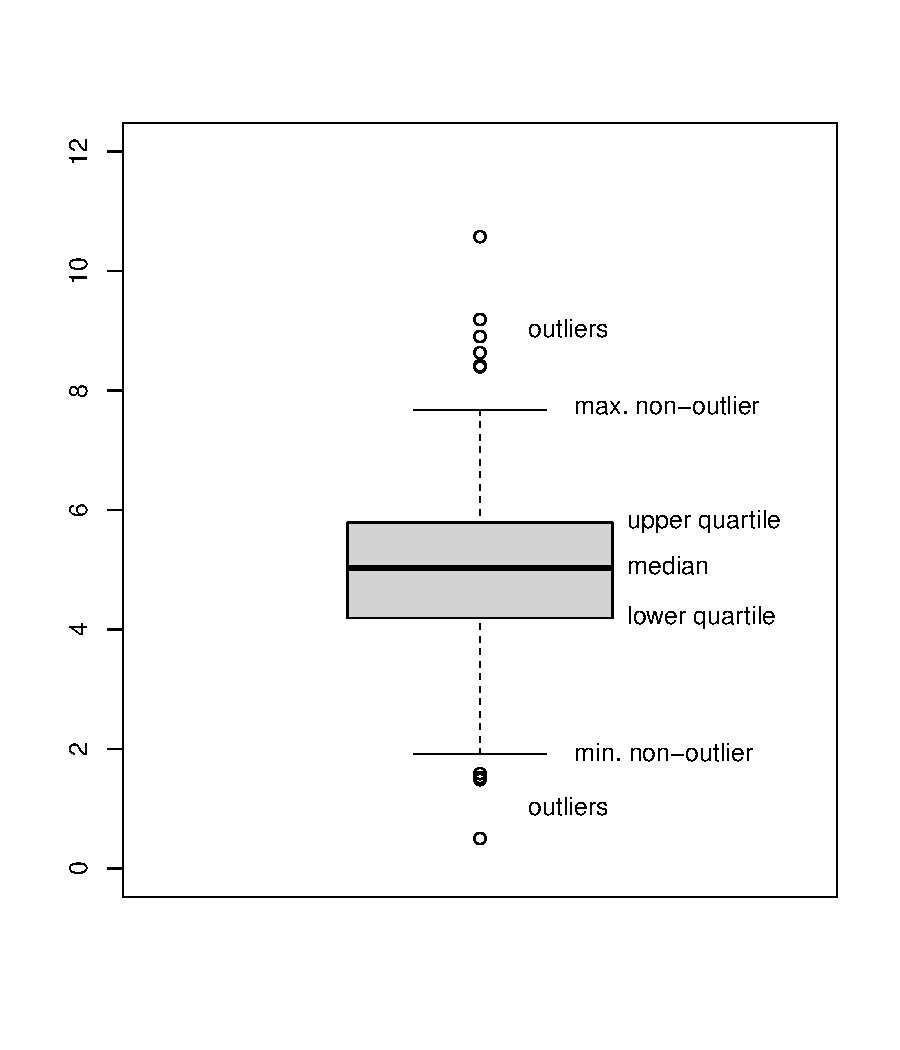
\includegraphics{math1710_files/figure-latex/boxplot1-1} \end{center}

When we have multiple datasets, drawing boxplots next to each other can help us to compare the datasets. Here are two boxplots from the July and October temperature data we used in the last lecture. What do you conclude about the data from these boxplots?

\begin{Shaded}
\begin{Highlighting}[]
\FunctionTok{boxplot}\NormalTok{(jul}\SpecialCharTok{$}\NormalTok{temp, oct}\SpecialCharTok{$}\NormalTok{temp,}
        \AttributeTok{names =} \FunctionTok{c}\NormalTok{(}\StringTok{"July"}\NormalTok{, }\StringTok{"October"}\NormalTok{),}
        \AttributeTok{ylab =} \StringTok{"Daily maximum temperature (degrees C) in Leeds"}
\NormalTok{)}
\end{Highlighting}
\end{Shaded}

\begin{center}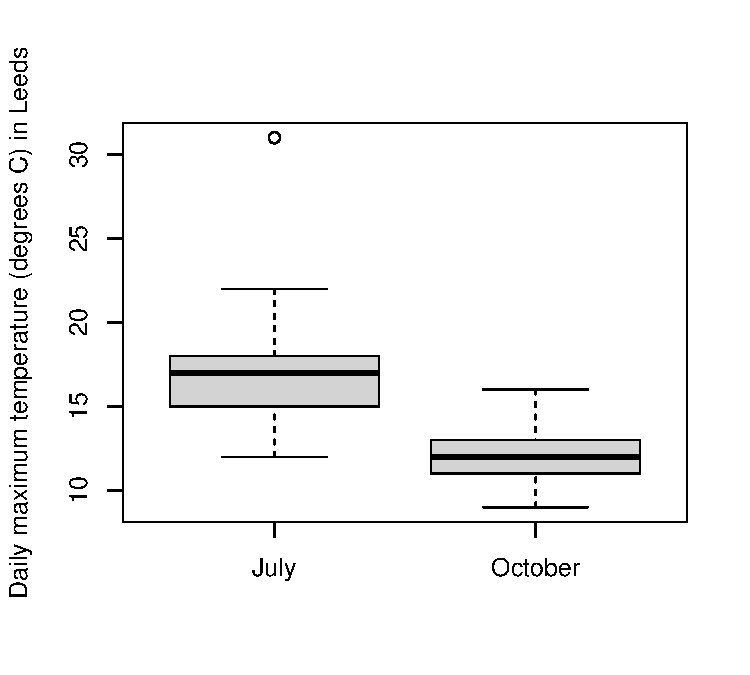
\includegraphics{math1710_files/figure-latex/boxplot-temp-1} \end{center}

(And yes, I \href{https://www.metoffice.gov.uk/binaries/content/assets/metofficegovuk/pdf/weather/learn-about/uk-past-events/interesting/2020/2020_05_july_temperature.pdf}{did check the outlier} to make sure it was a genuine datapoint.)

\hypertarget{histograms}{%
\section{Histograms}\label{histograms}}

Often when collecting data, we don't collect exact data, but rather collect data clumped into ``bins''. For example, suppose a student wished to use a questionnaire to collect data on how long it takes people to reach campus from home; they might not ask ``Exactly how long does it take?'', but rather give a choice of tick boxes: ``0--5 minutes'', ``5--10 minutes'', and so on.

Consider the following binned data, from \(n = 100\) students:

\begin{longtable}[]{@{}ccc@{}}
\toprule\noalign{}
Time & Frequency & Relative frequency \\
\midrule\noalign{}
\endhead
\bottomrule\noalign{}
\endlastfoot
0--5 minutes & 4 & 0.04 \\
5--10 minutes & 8 & 0.08 \\
10--15 minutes & 21 & 0.21 \\
15--30 minutes & 42 & 0.42 \\
30--45 minutes & 15 & 0.15 \\
45--60 minutes & 8 & 0.08 \\
60--120 minutes & 2 & 0.02 \\
\textbf{Total} & 100 & 1 \\
\end{longtable}

Here the \textbf{frequency} \(f_j\) of bin \(j\) is simply the number of observations in that bin; so, for example, 42 students had journey lengths of between 15 and 30 minutes. The \textbf{relative frequency} of bin \(j\) is \(f_j/n\); that is, the proportion of the observations in that bin.

Which bin would you say is the most popular -- that is, the ``modal'' bin? The bin with the most observations in it is the ``15--30 minute'' bin. But this bin covers 15 minutes, while some of the other bins only cover 5 minutes. It would be a fairer comparison to look at the \textbf{frequency density}: the relative frequency divided by the size of the bin.

\begin{longtable}[]{@{}cccc@{}}
\toprule\noalign{}
Time & Frequency & Relative frequency & Frequency density \\
\midrule\noalign{}
\endhead
\bottomrule\noalign{}
\endlastfoot
0--5 minutes & 4 & 0.04 & 0.008 \\
5--10 minutes & 8 & 0.08 & 0.016 \\
10--15 minutes & 21 & 0.21 & 0.042 \\
15--30 minutes & 42 & 0.42 & 0.028 \\
30--45 minutes & 15 & 0.15 & 0.010 \\
45--60 minutes & 8 & 0.08 & 0.005 \\
60--120 minutes & 2 & 0.02 & 0.0003 \\
\textbf{Total} & 100 & 1 & \\
\end{longtable}

In the first row, for example, the relative frequency is 0.04 and the size of the bin is 5 minutes, so the frequency density is \(0.04/5 = 0.008\). We now see that the modal bin -- the bin with the highest frequency \emph{density} -- is in fact the ``10--15 minutes'' bin. This bin has somewhat fewer datapoints that the ``15--30 minutes'' bin, but they're squashed into a much smaller bin.

Data in bins can be illustrated with a \textbf{histogram}. A histogram has the measurement on the x-axis, with one bar across the width of each bin, where bars are drawn up to the height of the corresponding frequency density. Note that this means that the area of the bar is exactly the relative frequency of the corresponding bin.

If all the bins are the same width, frequency density is directly proportional to frequency and to relative frequency, so it can be clearer use one of those as the y-axis instead in the equal-width-bins case.

Here is a histogram for our journey-time data:

\begin{Shaded}
\begin{Highlighting}[]
\NormalTok{journeys }\OtherTok{\textless{}{-}} \FunctionTok{read.csv}\NormalTok{(}\StringTok{"https://mpaldridge.github.io/math1710/data/journeys.csv"}\NormalTok{)}
\NormalTok{bins }\OtherTok{\textless{}{-}} \FunctionTok{c}\NormalTok{(}\DecValTok{0}\NormalTok{, }\DecValTok{5}\NormalTok{, }\DecValTok{10}\NormalTok{, }\DecValTok{15}\NormalTok{, }\DecValTok{30}\NormalTok{, }\DecValTok{45}\NormalTok{, }\DecValTok{60}\NormalTok{, }\DecValTok{120}\NormalTok{)}

\FunctionTok{hist}\NormalTok{(journeys}\SpecialCharTok{$}\NormalTok{midpoint, }\AttributeTok{breaks =}\NormalTok{ bins,}
     \AttributeTok{xlab =} \StringTok{"Journey length (min)"}\NormalTok{, }\AttributeTok{ylab =} \StringTok{"frequency density"}\NormalTok{, }\AttributeTok{main =} \StringTok{""}
\NormalTok{)}
\end{Highlighting}
\end{Shaded}

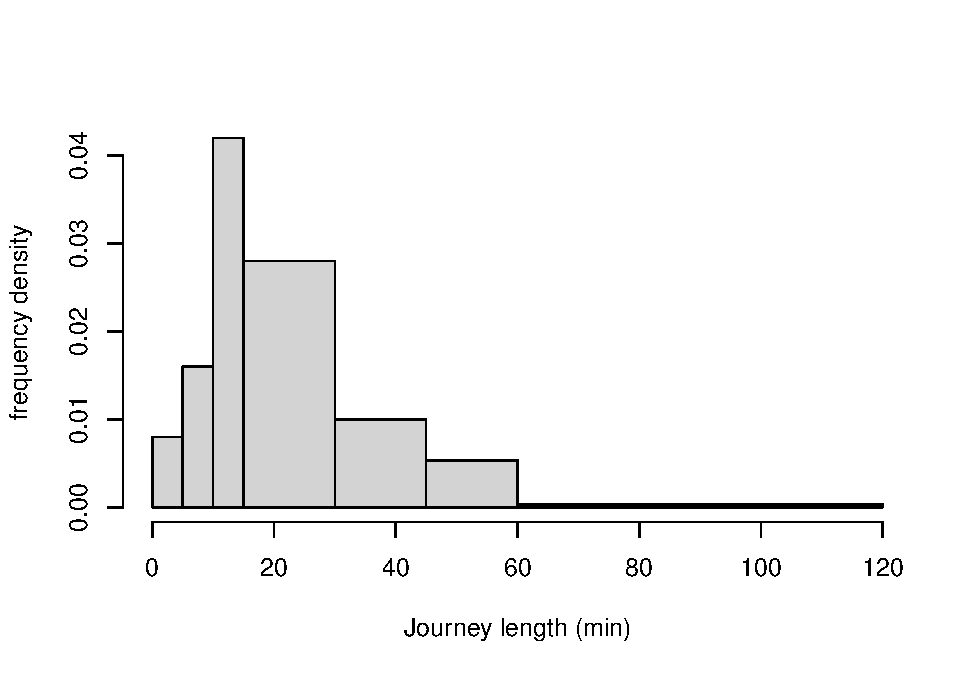
\includegraphics{math1710_files/figure-latex/journeys-1.pdf}

Often we draw histograms because the data was collected in bins in the first place. But even when we have exact data, we might \emph{choose} to divide it into bins for the purposes of drawing a histogram. In this case we have to decide where to put the ``breaks'' between the bins. Too many breaks too close together, and the small number of observations in each bin will give ``noisy'' results (see left); too few breaks too far apart, and the wide bins will mean we lose detail (see right).

\begin{Shaded}
\begin{Highlighting}[]
\FunctionTok{set.seed}\NormalTok{(}\DecValTok{2172}\NormalTok{)}
\NormalTok{hist\_data }\OtherTok{\textless{}{-}} \FunctionTok{c}\NormalTok{(}\FunctionTok{rnorm}\NormalTok{(}\DecValTok{30}\NormalTok{, }\DecValTok{8}\NormalTok{, }\DecValTok{2}\NormalTok{), }\FunctionTok{rnorm}\NormalTok{(}\DecValTok{40}\NormalTok{, }\DecValTok{12}\NormalTok{, }\DecValTok{3}\NormalTok{))  }\CommentTok{\# Some fake data}

\FunctionTok{hist}\NormalTok{(hist\_data, }\AttributeTok{breaks =} \DecValTok{40}\NormalTok{, }\AttributeTok{main =} \StringTok{"Too many bins"}\NormalTok{)}
\FunctionTok{hist}\NormalTok{(hist\_data, }\AttributeTok{breaks =} \DecValTok{2}\NormalTok{,  }\AttributeTok{main =} \StringTok{"Too few bins"}\NormalTok{)}
\end{Highlighting}
\end{Shaded}

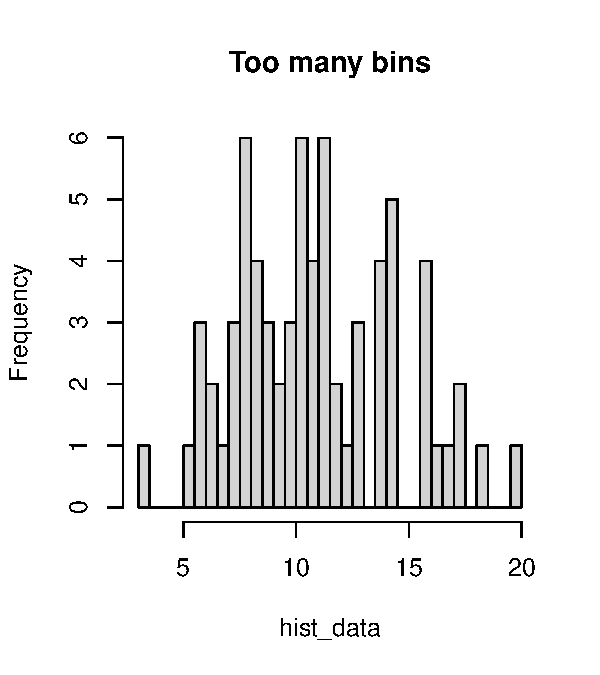
\includegraphics[width=0.48\linewidth]{math1710_files/figure-latex/hist-bins-1} 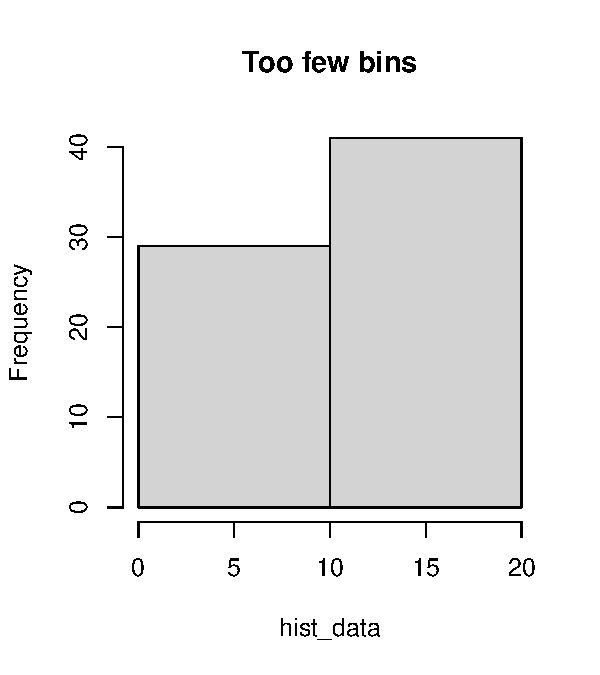
\includegraphics[width=0.48\linewidth]{math1710_files/figure-latex/hist-bins-2}

We can also calculate some summary statistics even when we have binned data. We mentioned the mode earlier, where the modal bin is the bin of highest frequency density.

What is the median journey length? Well, we don't know exactly, but \(0.04 + 0.08 + 0.21\) (the first three bins) is less than 0.5, while \(0.04 + 0.08 + 0.21 + 0.42\) (including the fourth bin) is greater than 0.5. So we know that the median student is in the fourth bin, the ``15--30 minute'' bin, and we can say that the median journey length is between 15 and 30 minutes.

Since we don't have the exact data, it's not possible to exactly calculate the mean and variance. However, we can often get a good estimate by assuming that each observation was in fact right in the centre of its bin. So, for example, we could assume that all 4 observations in the ``0--5 minutes'' bin were journeys of exactly 2.5 minutes. Of course, this isn't true (or is highly unlikely to be true), but we can often get a good approximation this way.

For our journey-time data, our approximation of the mean would be
\[ \bar x = \frac{1}{100} \big(4\times 2.5 + 8 \times 7.5 + \cdots + 2\times90) = 24.4 . \]
More generally, if \(m_j\) is the midpoint of bin \(j\) and \(f_j\) its frequency, then we can calculate the binned mean and binned variance by
\begin{align*}
  \bar x &= \frac{1}{n} \sum_j f_j m_j \\
  s^2_x  &= \frac{1}{n-1} \sum_j f_j (m_j - \bar x)^2
\end{align*}

\hypertarget{scatterplots}{%
\section{Scatterplots}\label{scatterplots}}

Often, more than one piece of data is collected from each subject, and we wish to compare that data, to see if there is a relationship between the variables.

For example, we could take \(n\) second-year maths students, and for each student \(i\), collect their mark \(x_i\) in MATH1710 and their mark \(y_i\) in MATH1712. This gives is two ``paired'' datasets, \(\mathbf x = (x_1, x_2, \dots, x_n)\) and \(\mathbf y = (y_1, y_2, \dots, y_n)\). We can calculate sample statistics of draw plots for \(\mathbf x\) and for \(\mathbf y\) individually. But we might also want to see if there is a relationship \emph{between} \(\mathbf x\) and \(\mathbf y\): Do students with high marks in MATH1710 also get high marks in MATH1712?

A good way to visualise the relationship between two variables is to use a \textbf{scatterplot}. In a scatterplot, the \(i\)th data pair \((x_i, y_i)\) is illustrated with a mark (such as a circle or cross) whose x-coordinate has the value \(x_i\) and whose y-coordinate has the value \(y_i\).

In the following scatterplot, we have \(n = 50\) datapoints for the 50 US states; for each state \(i\), \(x_i\) is the Republican share of the vote in that state in the 2016 Trump--Clinton presidential election, and \(y_i\) is the Republican share of the vote in that state in the 2020 Trump--Biden election.

\begin{Shaded}
\begin{Highlighting}[]
\NormalTok{elections }\OtherTok{\textless{}{-}} \FunctionTok{read.csv}\NormalTok{(}\StringTok{"https://mpaldridge.github.io/math1710/data/elections.csv"}\NormalTok{)}

\FunctionTok{plot}\NormalTok{(elections}\SpecialCharTok{$}\NormalTok{X2016, elections}\SpecialCharTok{$}\NormalTok{X2020,}
     \AttributeTok{col =} \StringTok{"blue"}\NormalTok{,}
     \AttributeTok{xlab =} \StringTok{"Republican share of the two{-}party vote, 2016 (\%)"}\NormalTok{,}
     \AttributeTok{ylab =} \StringTok{"Republican share of the two{-}party vote, 2020 (\%)"}\NormalTok{)}

\FunctionTok{abline}\NormalTok{(}\AttributeTok{h =} \DecValTok{50}\NormalTok{, }\AttributeTok{col =} \StringTok{"grey"}\NormalTok{)}
\FunctionTok{abline}\NormalTok{(}\AttributeTok{v =} \DecValTok{50}\NormalTok{, }\AttributeTok{col =} \StringTok{"grey"}\NormalTok{)}
\FunctionTok{abline}\NormalTok{(}\FloatTok{0.195}\NormalTok{, }\FloatTok{0.963}\NormalTok{, }\AttributeTok{col =} \StringTok{"red"}\NormalTok{)}
\end{Highlighting}
\end{Shaded}

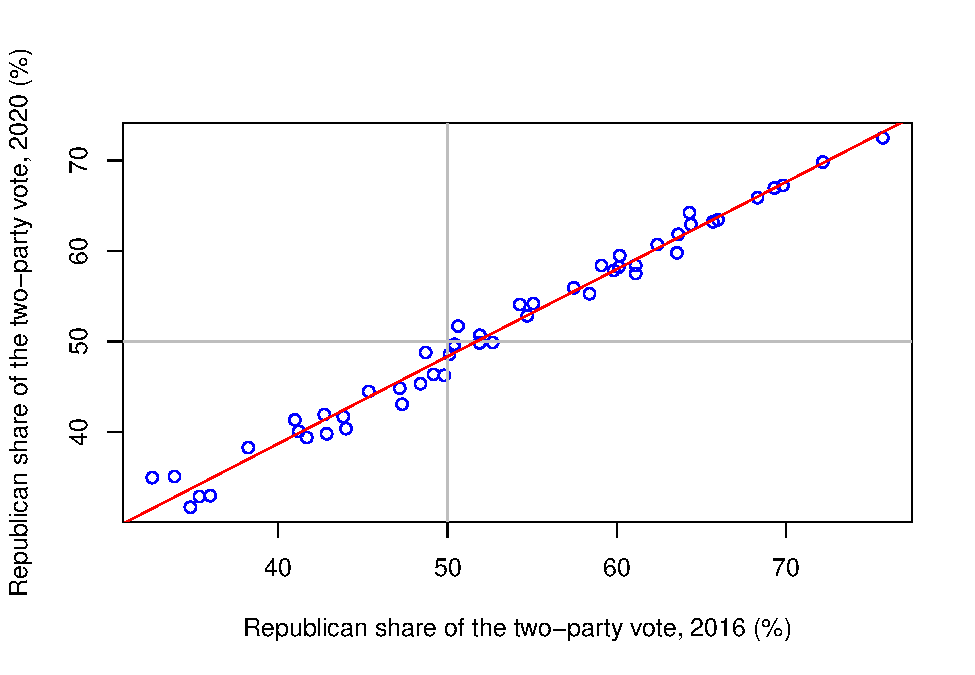
\includegraphics{math1710_files/figure-latex/elections-1.pdf}

We see that there is a strong relationship between \(\mathbf x\) and \(\mathbf y\), with high values of \(x\) corresponding to high values of \(y\) and vice versa. Further, the points on the scatterplot lie very close to a straight line.

A useful summary statistic here is the \textbf{correlation}
\[ r_{xy} = \frac{s_{xy}}{s_x s_y} , \]
where \(s_{xy}\) is the \textbf{sample covariance}
\begin{align*}
s_{xy} &= \frac{1}{n-1} \big( (x_1 - \bar x)(y_1 - \bar y) + \cdots + (x_n - \bar x)(y_n - \bar y) \big) \\
  &= \frac{1}{n-1} \sum_{i=1}^n (x_i - \bar x)(y_i - \bar y) ,
\end{align*}
and \(s_x = \sqrt{s_x^2}\) and \(s_y = \sqrt{s_y^2}\) are the standard deviations.

The correlation \(r_{xy}\) is always between \(-1\) and \(+1\). Values of \(r_{xy}\) near \(+1\) indicate that the scatterpoints are close to a straight line with an upward slope (big \(x\) = big \(y\)); values of \(r_{xy}\) near \(-1\) indicate that the scatterpoints are close to a straight line with a downward slope (big \(x\) = small \(y\)); and values of \(r_{xy}\) near 0 indicate that there is a weak linear relationship between \(x\) and \(y\).

For the elections data, the correlation is

\begin{Shaded}
\begin{Highlighting}[]
\FunctionTok{cor}\NormalTok{(elections}\SpecialCharTok{$}\NormalTok{X2016, elections}\SpecialCharTok{$}\NormalTok{X2020)}
\end{Highlighting}
\end{Shaded}

\begin{verbatim}
[1] 0.9919659
\end{verbatim}

which, as we expected, is extremely high.

\hypertarget{summary-02}{%
\section*{Summary}\label{summary-02}}
\addcontentsline{toc}{section}{Summary}

\begin{itemize}
\tightlist
\item
  Boxplots show the shape of numerical data, and can compare different datasets.
\item
  Histograms show the shape of binned data.
\item
  Scatterplots show the relationship between two datasets.
\end{itemize}

\textbf{Recommended reading:}

\begin{itemize}
\tightlist
\item
  Wikipedia: \href{https://en.wikipedia.org/wiki/Box_plot}{Box plot}, \href{https://en.wikipedia.org/wiki/Histogram}{Histogram}, \href{https://en.wikipedia.org/wiki/Grouped_data}{Grouped data}, \href{https://en.wikipedia.org/wiki/Scatter_plot}{Scatter plot}, \href{https://en.wikipedia.org/wiki/Pearson_correlation_coefficient}{Pearson correlation coefficient}.
\item
  Clarke and Cooke, \emph{A Basic Course in Statistics}, Sections 1.2, 2.5, 4.5, 4.6, 21.2, 21.3.
\end{itemize}

On \protect\hyperlink{P1}{Problem Sheet 1}, you should now be able to complete all questions.

\hypertarget{P1}{%
\chapter*{Problem Sheet 1}\label{P1}}
\addcontentsline{toc}{chapter}{Problem Sheet 1}

\commfalse

\protect\hyperlink{P1-solutions}{\textbf{Solutions} are now available} to all non-assessed questions.

You can \href{P1-sheet.pdf}{download this problem sheet as a PDF file}

This is Problem Sheet 1, which covers material from Lectures \protect\hyperlink{L01-stats}{1} and \protect\hyperlink{L02-dataviz}{2} of the notes. You should work through all the questions on this problem sheet in advance of your tutorial in Week 2. Questions C1 and C2 are assessed questions, and are due in by \textbf{2pm on Monday 16 October}. I recommend spending about 4 hours on this problem sheet, plus 1 extra hour to neatly write up and submit your answers to the assessed questions.

\hypertarget{P1-short}{%
\section*{A: Short questions}\label{P1-short}}
\addcontentsline{toc}{section}{A: Short questions}

The first three questions are \textbf{short questions}, which are intended to be mostly not too difficult. Short questions usually follow directly from the material in the lectures. Here, you should clearly state your final answer, and give enough working-out (or a short written explanation) for it to be clear how you reached that answer. You can check your answers with the solutions-without-working at the bottom of this sheet; solutions-with-working will be available after Friday 13 October. If you get stuck on any of these questions, you might want to ask for guidance in your tutorial.

\textbf{A1.} Consider again the ``number of Skittles in each packet'' data from Example 1.1.
\[ 59, \ 59, \ 59, \ 59, \ 60, \ 60, \ 60, \ 61, \ 62, \ 62, \ 62, \ 63, \ 63 .\]

\textbf{(a)} Calculate the mean number of Skittles in each packet.

\begin{myanswers}
\emph{Solution.} This was in the notes:
\[ \bar x = \frac{1}{13} (59 + 59 + \cdots + 63) =  \frac{789}{13} = 60.6923\dots \approx 60.7 .\]

\end{myanswers}

\textbf{(b)} Calculate the sample variance using the definitional
formula.

\begin{myanswers}
\emph{Solution.}
\begin{align*}
s_x^2 &= \frac{1}{13 - 1} \left( (59 - 60.7)^2 + (59 - 60.7)^2 + \cdots + (63 - 60.7)^2 \right) \\
      &= \frac{1}{12} (2.86 + 2.86 + \cdots + 5.33) \\
      &= \frac{1}{12} \times 28.77 \\
      &= 2.40
\end{align*}

\end{myanswers}

\textbf{(c)} Calculate the sample variance using the computational formula.

\begin{myanswers}
\emph{Solution.}
\begin{align*}
s_x^2 &= \frac{1}{13 - 1} \left( (59^2 + 59^2 + \cdots + 63^2) - 13 \times 60.6923^2)\right) \\
      &= \frac{1}{12} (47915 - 47886.2) \\
      &= 2.40
\end{align*}

\textbf{Group feedback:} With the computational formula, the value \(\sum_i x_i^2 - n \bar{x}^2\) is typically a fairly small number given as the difference between two very big numbers \(\sum_i x_i^2\) and \(n \bar x^2\). This means you have to get the two big numbers very precise, to ensure the cancellation happens correctly; in particular, make sure you use plenty of decimal places of accuracy in \(\bar x\).

\end{myanswers}

\textbf{(d)} Out of (b) and (c), which calculation did you find easier, and why?

\begin{myanswers}
\emph{Solution.} The computational formula required fewer presses of the calculator buttons, because \(\sum_i x_i^2\) is fewer button-presses than \(\sum_i (x_i - \bar x)^2\), where you have to subtract the means before squaring.

On the other hand, the expression inside the brackets of the computational formula is a fairly small number given as the difference of two very large numbers, so it was necessary to use lots of decimal places of accuracy in \(\bar x\) to make sure the second large number was accurate and therefore that the subtraction cancelled correctly.

\textbf{Group feedback:} Many different answers for (d) are fine provided you give a justification.

\end{myanswers}

\textbf{A2.} Consider the following data sets of the age of elected politicians on a local council. (The ``18--30'' bin, for example, means from one's
18th birthday to the moment before one's 30th birthday, so lasts 12 years.)

\begin{longtable}[]{@{}
  >{\centering\arraybackslash}p{(\columnwidth - 6\tabcolsep) * \real{0.2537}}
  >{\centering\arraybackslash}p{(\columnwidth - 6\tabcolsep) * \real{0.1642}}
  >{\centering\arraybackslash}p{(\columnwidth - 6\tabcolsep) * \real{0.2985}}
  >{\centering\arraybackslash}p{(\columnwidth - 6\tabcolsep) * \real{0.2836}}@{}}
\toprule\noalign{}
\begin{minipage}[b]{\linewidth}\centering
Age (years)
\end{minipage} & \begin{minipage}[b]{\linewidth}\centering
Frequency
\end{minipage} & \begin{minipage}[b]{\linewidth}\centering
Relative frequency
\end{minipage} & \begin{minipage}[b]{\linewidth}\centering
Frequency density
\end{minipage} \\
\midrule\noalign{}
\endhead
\bottomrule\noalign{}
\endlastfoot
18--30 & 1 & & \\
30--40 & 2 & & \\
40--45 & 4 & & \\
45--50 & 5 & & \\
50--60 & 6 & & \\
60--80 & 2 & & \\
\textbf{Total} & 20 & 1 & --- \\
\end{longtable}

\textbf{(a)} Complete the table by filling in the relative frequency and
frequency densities.

\begin{myanswers}

\emph{Solution.}

\begin{longtable}[]{@{}
  >{\centering\arraybackslash}p{(\columnwidth - 6\tabcolsep) * \real{0.2537}}
  >{\centering\arraybackslash}p{(\columnwidth - 6\tabcolsep) * \real{0.1642}}
  >{\centering\arraybackslash}p{(\columnwidth - 6\tabcolsep) * \real{0.2985}}
  >{\centering\arraybackslash}p{(\columnwidth - 6\tabcolsep) * \real{0.2836}}@{}}
\toprule\noalign{}
\begin{minipage}[b]{\linewidth}\centering
Age (years)
\end{minipage} & \begin{minipage}[b]{\linewidth}\centering
Frequency
\end{minipage} & \begin{minipage}[b]{\linewidth}\centering
Relative frequency
\end{minipage} & \begin{minipage}[b]{\linewidth}\centering
Frequency density
\end{minipage} \\
\midrule\noalign{}
\endhead
\bottomrule\noalign{}
\endlastfoot
18--30 & 1 & 0.05 & 0.0042 \\
30--40 & 2 & 0.1 & 0.01 \\
40--45 & 4 & 0.2 & 0.04 \\
45--50 & 5 & 0.25 & 0.05 \\
50--60 & 6 & 0.3 & 0.03 \\
60--80 & 2 & 0.1 & 0.005 \\
\textbf{Total} & 20 & 1 & --- \\
\end{longtable}

\end{myanswers}

\textbf{(b)} What is the median age bin?

\begin{myanswers}
\emph{Solution.} The 10th- and 11th-largest observations are both in the 45--50 bin, which is therefore the median bin.

\end{myanswers}

\textbf{(c)} What is the modal age bin?

\begin{myanswers}
\emph{Solution.} The bin with the largest frequency density is 45--50, which is therefore the modal bin.

\textbf{Group feedback:} Remember that the modal bin is the one with the largest frequency \emph{density}, not necessarily the bin with the highest frequency.

\end{myanswers}

\textbf{(d)} Calculate (the standard approximation of) the mean age of the politicians.

\begin{myanswers}
\emph{Solution.} Pretending that each person is in the centre of their bin, we have
\[ \bar x = \frac{1}{20} (1\times24 + 2\times 35 + \cdots + 2 \times 65) = \frac{971.9}{20} = 48.6 . \]

\end{myanswers}

\textbf{A3.} Consider the two datasets illustrated by the boxplots below. Write down some differences between the two datasets.

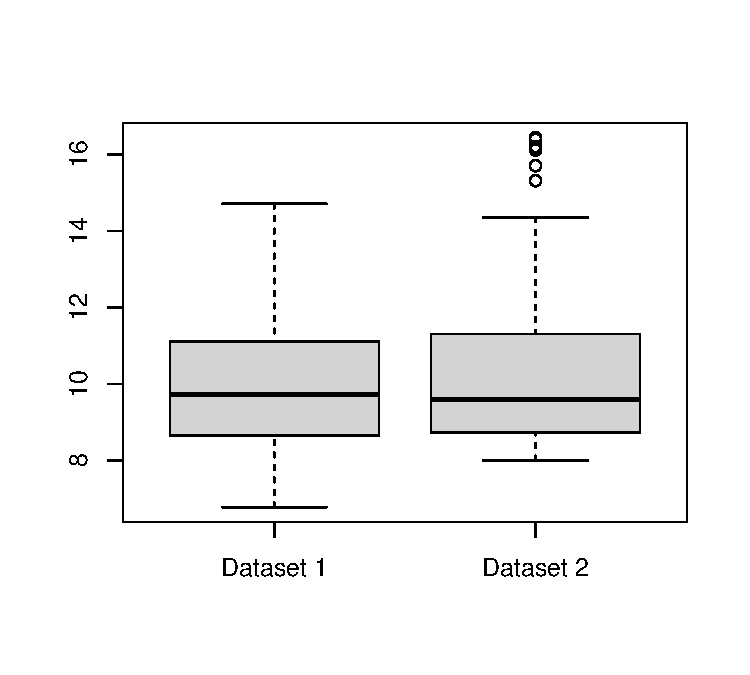
\includegraphics{math1710_files/figure-latex/unnamed-chunk-16-1.pdf}

\begin{myanswers}
\emph{Solution.} Some answers could be:

\begin{itemize}
\tightlist
\item
  The median and inter-quartile range of Dataset 2 appear to be very slightly larger than those in Dataset 1, although the differences are very small and might not be important in real life.
\item
  Dataset 2 has a few outliers; Dataset 1 has none.
\item
  While Dataset 1 is fairly ``balanced'' either side of the median, Dataset 2 shows what statisticians call a ``positive skew'': the data above the median is much more spread out than the data below the median.
\end{itemize}

\textbf{Group feedback:}
You can probably think of other answers.

\end{myanswers}

\hypertarget{P1-long}{%
\section*{B: Long questions}\label{P1-long}}
\addcontentsline{toc}{section}{B: Long questions}

The next four questions are \textbf{long questions}, which are intended to be harder. Long questions often require you to think originally for yourself, not just directly follow procedures from the notes. You may not be able to solve all of these questions, although you should make multiple attempts to do so. Here, your answers should be written in complete sentences, and you should carefully explain in words each step of your working. Your answers to these questions -- not only their mathematical content, but also how to write good, clear solutions -- are likely to be the main topic for discussion in your tutorial. Solutions will be available after Friday 13 October.

\textbf{B1.} For each of the two datasets below, calculate the following summary statistics, or explain why it is not possible to do so: mode; median; mean; number of distinct outcomes; inter-quartile range; and sample variance.

\textbf{(a)} Shirt sizes for the \(n = 16\) members of a university football squad:

\begin{longtable}[]{@{}
  >{\centering\arraybackslash}p{(\columnwidth - 10\tabcolsep) * \real{0.3333}}
  >{\centering\arraybackslash}p{(\columnwidth - 10\tabcolsep) * \real{0.1667}}
  >{\centering\arraybackslash}p{(\columnwidth - 10\tabcolsep) * \real{0.1111}}
  >{\centering\arraybackslash}p{(\columnwidth - 10\tabcolsep) * \real{0.1111}}
  >{\centering\arraybackslash}p{(\columnwidth - 10\tabcolsep) * \real{0.1111}}
  >{\centering\arraybackslash}p{(\columnwidth - 10\tabcolsep) * \real{0.1667}}@{}}
\toprule\noalign{}
\begin{minipage}[b]{\linewidth}\centering
\textbf{Colour}
\end{minipage} & \begin{minipage}[b]{\linewidth}\centering
Xtra Small
\end{minipage} & \begin{minipage}[b]{\linewidth}\centering
Small
\end{minipage} & \begin{minipage}[b]{\linewidth}\centering
Medium
\end{minipage} & \begin{minipage}[b]{\linewidth}\centering
Large
\end{minipage} & \begin{minipage}[b]{\linewidth}\centering
Xtra Large
\end{minipage} \\
\midrule\noalign{}
\endhead
\bottomrule\noalign{}
\endlastfoot
\textbf{Number of shirts} & 0 & 1 & 6 & 4 & 5 \\
\end{longtable}

\begin{myanswers}
\emph{Solution.}
The modal shirt size is medium. The number of distinct outcomes is 4 (we don't quite ``Xtra Small'', which was not observed in the data).

This time, we can order the data from smallest to largest, even though the data is not numerical. Since \((16 + 1)/2 - 8.5\), the median datapoint is the 8th or 9th datapoints, which are Large.

Since \(1 + 0.25(16 - 1) = 4.75\) the lower quartile is the 4th or 5th datapoints, which are Medium. Since \(1 + 0.75(16-1) = 12.25\), the upper quartile is the 12th or 13th datapoints, which are Xtra Large. So we can certainly say that the inner quartiles range from Medium to Xtra Large. We could probably also say that the interquartile range is 3 shirt sizes (Medium, Large, Xtra Large).

Again, because the data is not numerical, we can't add it up, so can't calculate a mean or sample variance.

\end{myanswers}

\textbf{(b)} Six packets of Skittles are opened together, a total of \(n = 361\) sweets. The colours of these sweets is recorded as follows:

\begin{longtable}[]{@{}cccccc@{}}
\toprule\noalign{}
\textbf{Colour} & Red & Orange & Yellow & Green & Purple \\
\midrule\noalign{}
\endhead
\bottomrule\noalign{}
\endlastfoot
\textbf{Number of Skittles} & 67 & 71 & 87 & 74 & 62 \\
\end{longtable}

\begin{myanswers}
\emph{Solution.}
The modal colour is Yellow. The number of distinct outcomes is 5.

It's not possible to calculate the median or the quartiles, because, unlike numerical data, the colours can't be put ``in order'' from smallest to largest.

It's not possible to calculate the mean or sample variance, as these require us to have numerical data that can be ``added up'', but this can't be done with colours.

\textbf{Group feedback:} Make sure your explanation is clear for why we can't calculate a median for the Skittles data but can for the shirts: the key is whether or not the data can be \emph{ordered}.

\end{myanswers}

\textbf{B2.} A summary statistic is informally said to be ``robust'' if it typically doesn't change much if a small number of outliers are introduced to a large dataset, or ``sensitive'' if it often changes a lot when a small number of outliers are introduced. Briefly discuss the robustness or sensitivity of the following summary statistics: \textbf{(a)} mode; \textbf{(b)} median; \textbf{(c)} mean; \textbf{(d)} number of distinct outcomes; \textbf{(e)} inter-quartile range; and \textbf{(f)} sample variance.

\begin{myanswers}
\emph{Solutions.}

\textbf{(a)} An outlier will typically be the only data point with its value, or certainly rare. Therefore, the mode will typically not change at all if a small number of outliers are introduced, so is robust. (The exception is for data where every observation is likely to be different, so any outliers become ``joint modes'' along with everything else; but in this case the mode is not a useful statistic in the first place.)

\textbf{(b)} The introduction of outliers will typically only change the median a little bit, by shifting it between different nearby values in the ``central mass'' of the data. In particular, the \emph{size} of the outliers won't make any difference at all (only whether they are ``high outliers'' above the median or ``low outliers'' below the median). So the median is robust.

\textbf{(c)} The mean can change a lot if outliers are introduced, especially if the outlier is enormously far our from the data. So the mean is sensitive.

\textbf{(d)} The number of distinct outcomes will only increase by (at most) 1 for each outlier introduced. This is not typically a relevant increase, so the number of distinct outcomes is robust.

\textbf{(e)} The interquartile range is robust, for the same reason as the median.

\textbf{(f)} The sample variance is sensitive, for the same reason as the mean.

(You might like to think about situations where it's better to use a robust statistic or better to use a sensitive statistic.)

\textbf{Group feedback:} I find it helpful to suppose I was studying the net worth of people in my tutorial group, and calculating summary statistics. How would those statistics changed change if Elon Musk (owner of Tesla and Twitter, net worth roughly \$200 billion) joined my tutorial group? The mean and sample variance would change an enormous amount, while the median and interquartile range would barely change at all in comparison.

Remember that ``robust'' and ``sensitive'' are general descriptions rather than precise mathematical definitions. So it doesn't matter if you disagree with my opinions provided that you give clear and detailed explanations to back up your opinion.

\end{myanswers}

\textbf{B3.} Let \(\mathbf a = (a_1, a_2, \dots a_n)\) and \(\mathbf b = (b_1, b_2, \dots, b_n)\) be two real-valued vectors of the same length. Then the \emph{Cauchy--Schwarz inequality} says that
\[ \left( \sum_{i=1}^n a_i b_i \right)^2 \leq \left( \sum_{i=1}^n a_i^2 \right) \left(\sum_{i=1}^n b_i^2 \right) . \]

\textbf{(a)} By making a clever choice of \((a_i)\) and \((b_i)\) in the Cauchy--Schwarz inequality, show that \(s_{xy}^2 \leq s_x^2 s_y^2\).

\begin{myanswers}
\emph{Solutions.}
Recalling the formulas for \(s_{xy}\), \(s_x^2\), and \(s_y^2\),
\begin{align*}
s_{xy} &= \frac{1}{n-1} \sum_{i=1}^n (x_i - \bar x)(y_i - \bar y) ,\\
s_{x}^2 &= \frac{1}{n-1} \sum_{i=1}^n (x_i - \bar x)^2 ,\\
s_{y}^2 &= \frac{1}{n-1} \sum_{i=1}^n (y_i - \bar y)^2 ,
\end{align*}
and comparing them with the Cauchy--Schwarz inequality, it looks like taking \(a_i = x_i - \bar x\) and \(b_i = y_i - \bar y\) might be useful.

Making that substitution, we get
\[ \left( \sum_{i=1}^n (x_i - \bar x)(y_i - \bar y) \right)^2 \leq \left( \sum_{i=1}^n (x_i - \bar x)^2 \right) \left(\sum_{i=1}^n (y_i - \bar y)^2 \right) . \]

These are very close to the formulas for \(s_{xy}\), \(s_x^2\), and \(s_y^2\), but are just missing the ``\(1/(n-1)\)''s; what we in fact have is
\[ \left( (n-1) s_{xy} \right)^2 \leq (n-1)s_x^2 \cdot (n-1) s_y^2 .\]
Cancelling \((n-1)^2\) from each side, we have \(s_{xy}^2 \leq s_x^2 s_y^2\), as required.

\textbf{Group feedback:} Keep trying different choices for \((a_i)\) and \((b_i)\); maybe your first attempt won't work, but it pays to be persistent!

A fancier choice is \(a_i = (x_i - \bar x)/\sqrt{n-1}\) and \(b_i = (y_i - \bar y)/\sqrt{n-1}\), to get the exact result without needing a second cancellation step, but I would find that harder to spot.

\end{myanswers}

\textbf{(b)}
Hence, show that the correlation \(r_{xy}\) satisfies \(-1 \leq r_{xy} \leq 1\).

\begin{myanswers}
\emph{Solutions.}
Recall the formula for the correlation is
\[ r_{xy} = \frac{s_{xy}}{s_xs_y} . \]
We can make part (a) look a bit like this dividing both sides by \(s_x^2 s_y^2\), to get
\[\frac{s_{xy}^2}{s_x^2 s_y^2} \leq 1.   \]
In fact that's the square of the correlation on the left-hand side, so we've shown that \(r_{xy}^2 \leq 1\).

Finally, we note that if a number squared is less than or equal to 1, then the number must be between -1 and +1 inclusive. (Numbers bigger than 1 get bigger still when squared; numbers smaller than -1 become bigger than +1 when squared; numbers between -1 and +1 get closer to 0.) Hence we have shown that \(-1 \leq r_{xy} \leq 1\), as required.

\textbf{Group feedback:} In part (b) there's a temptation to ``square-root both sides of the inequality''. But you have to be extremely careful if you do this -- make sure you are properly accounting for the positive and negative square roots on both sides (if necessary), and where that does or doesn't require reversing the direction of the inequality. I recommend leaving the square-root operation until the last possible moment of the proof or, perhaps even better, reasoning through words as I did above.

Remember that you can still attempt part (b) even if you got stuck on part (a).

\end{myanswers}

\textbf{B4.} A researcher wishes to study the effect of mental health on academic achievement. The researcher will collect data on the mental health of a cohort of students by asking them to fill in a questionnaire, and will measure academic achievement via the students' scores on their university exams. Discuss some of the ethical issues associated with the collection, storage, and analysis of this data, and with the publication of the results of the analysis. Are there ways to mitigate these issues?

(It's not necessary to write an essay for this question -- a few short bulletpoints will suffice. There may be an opportunity to discuss these issues in more detail in your tutorial.)

\begin{myanswers}
\textbf{Group feedback:} There are no ``correct'' or ``incorrect'' answers here, but here are a few things that students in my own tutorials brought up, which may act as a prompt for your own discussions.

\begin{itemize}
\item
  It's important the students/subjects have given their consent for their data to be used this way. It must be ``informed consent'', where they understand for what purpose the data will be used, how it will be stored, and so on. It must be easy and painless for students to decline to take part.
\item
  Consideration should be given on how to anonymise the data as much as possible -- it's not necessary for those analysing the data to know which questionnaire or which exam result belongs to which student, only that the questionnaire and results can be paired up.
\item
  Even if after data is anonymised, care should be taken about whether the students could be worked out from the data. For example, if only one student did a certain combination of modules, their identity could ``leak'' that way. Perhaps imprecise data, such as classes rather than exact marks, might help maintain privacy while only slightly reducing the usefulness of the data?
\item
  On one hand, it seems like this data should perhaps be deleted once analysis has been carried out, for the privacy of the students. On the other hand, principles of ``open science'' suggest that the data should be kept -- and even publicly made available -- for other researchers to check the work. There are competing ethical considerations here.
\item
  If correlations are found in the data, care should be taken when publishing the analysis not to wrongly suggest a causation. (Just because X and Y are positively correlated, it doesn't mean that X \emph{causes} Y -- or that Y causes X.)
\end{itemize}

You can probably think of many other things.

\end{myanswers}

\hypertarget{P1-assessed}{%
\section*{C: Assessed questions}\label{P1-assessed}}
\addcontentsline{toc}{section}{C: Assessed questions}

The last two questions are \textbf{assessed questions}. This means you will submit your answers, and your answers will be marked by your tutor. These two questions count for 3\% of your final mark for this module. If you get stuck, your tutor may be willing to give you a small hint in your tutorial.

The deadline for submitting your solutions is \textbf{2pm on Monday 16 October} at the beginning of Week 3. Submission will be via Gradescope, which you can access via Minerva or on the Gradescope mobile app.
You should submit your answers as a single PDF file. Most students choose to hand-write their work on paper, then scan-and-submit it to using the Gradescope mobile app. Your work will be marked by your tutor and returned on Monday 23 October, when solutions will also be made available.

Question C1 is a ``short question'', where brief explanations or working are sufficient; Question C2 is a ``long question'', where the marks are not only for mathematical accuracy but also for the clarity and completeness of your explanatory writing.

You should not collaborate with others on the assessed questions: your answers must represent solely your own work. The University's rules on \href{https://library.leeds.ac.uk/info/1401/academic_skills/46/academic_integrity_and_plagiarism}{academic integrity} -- and the related punishments for violating them -- apply to your work on the assessed questions.

\textbf{C1.} The monthly average exchange rate for US dollars into British pounds over a 12-month period was:
\begin{gather*}
1.306, \ 1.301, \ 1.290, \ 1.266, \ 1.268, \ 1.302,\\
1.317, \ 1.304, \ 1.284, \ 1.268, \ 1.247, \ 1.215.
\end{gather*}

\textbf{(a)} Calculate the median for this data.

\textbf{(b)} Calculate the mean for this data.

\textbf{(c)} Calculate the sample variance for this data.

\begin{myanswers}
\emph{Hints.}
Have you checked the definitions of these statistics from Subsection 1.3 of the notes?

\end{myanswers}

\textbf{(d)} Is the mode an appropriate summary statistic for this sort of data? Why/why not?

\begin{myanswers}
\emph{Hint.}
Is there a unique mode for this data? Why/why not? For what sort of data does the ``mode'' give us useful answers?

\end{myanswers}

\textbf{C2.}
~\textbf{(a)} Suppose that a dataset \(\mathbf x = (x_1, x_2, \dots, x_n)\) (with \(n \geq 2\)) has sample variance \(s_x^2 = 0\). Show that all the datapoints are in fact equal.

\begin{myanswers}
\emph{Hint.}
I recommend starting with the definitional formula.

When is the square of something equal to 0? What can you say about the value of a square when it's nonzero? What can you say about a ``sum of squares'' -- that is, some numbers squared then added together?

\end{myanswers}

\textbf{(b)} Prove the following computational formula for the sample covariance:
\[ s_{xy} = \frac{1}{n-1} \left( \sum_{i=1}^n x_iy_i - n\bar x \bar y \right). \]

\begin{myanswers}
\emph{Hint.}
In Subsection 1.4 of the notes, we went from the definitional formula for the sample \emph{variance} to a computational formula. Can you follow a similar argument here?

\end{myanswers}

\hypertarget{P1-short-sols}{%
\section*{Solutions to short questions}\label{P1-short-sols}}
\addcontentsline{toc}{section}{Solutions to short questions}

\textbf{A1.} (a) 60.7, (b) 2.40, (c) 2.40, (d) ---.\\
\textbf{A2.} (a) ---, (b) 45--50, (c) 45--50, (d) 48.6 \emph{(corrected)}.\\
\textbf{A3.} ---

\hypertarget{part-part-ii-probability}{%
\part*{Part II: Probability}\label{part-part-ii-probability}}
\addcontentsline{toc}{part}{Part II: Probability}

\hypertarget{L03-events}{%
\chapter{Sample spaces and events}\label{L03-events}}

\renewcommand{\complement}{\mathsf{c}}
\newcommand{\comp}{\complement}
\newcommand{\ff}[2]{{#1}^{\underline{#2}}}

\hypertarget{what-is-prob}{%
\section{What is probability?}\label{what-is-prob}}

We now begin the big central block of this module, on probability theory.

Probability theory is the study of randomness. Probability, as an area of mathematics, is a fascinating subject in its own right. However, probability is particularly important due to its usefulness in applications -- especially in statistics (the study of data), in finance, and in actuarial science (the study of insurance).

Probability is well suited to modelling situations that involve randomness, uncertainty, or unpredictability. If you want to predict the time of the next solar eclipse, a deterministic (that is, non-random) model based on physical laws will tell you when the sun, the moon, and the earth will be in the correct positions; but if you want to predict the weather tomorrow, or the price of a share of Apple stock next month, or the results of an election next year, you will need a probabilistic model that takes into account the uncertainty in the outcome. A probabilistic model could tell you the most likely outcome, or a range of the most probable outcomes.

So what do we mean when we talk about the ``probability'' of an event occurring? You might say that the probability of an event is a measure of ``how likely'' it is to occur, or what the ``chance'' of it occurring is.

More concretely, here are some interpretations of probability:

\begin{itemize}
\tightlist
\item
  \textbf{Subjective} (or \textbf{Bayesian}) \textbf{probability:} The probability of an event is the way someone expresses their degree of belief that the event will occur, based on their own judgement, and given the evidence they have seen. Their belief is measured on a scale from 0 to 1, from probabilities near 0 meaning they believe the event is very unlikely to occur to probabilities near 1 meaning they believe the event is very likely to occur.

  \begin{itemize}
  \tightlist
  \item
    This interpretation is philosophically sound, but a bit vague to be the basis for a mathematics module.
  \end{itemize}
\item
  \textbf{Classical} (or \textbf{enumerative}) \textbf{probability:} Suppose there are a finite number of equally likely outcomes. Then the probability of an event is the proportion of those outcomes that correspond to the event occurring. So when we say that a randomly dealt card has a probability \(\frac{1}{13}\) of being an ace, this is because there are 52 cards of which 4 are aces, so the proportion of favourable outcomes is \(\frac{4}{52} = \frac{1}{13}\).

  \begin{itemize}
  \tightlist
  \item
    This interpretation is good for simple procedures like flipping a fair coin, rolling a dice, or dealing cards, where the ``finite number of equally likely outcomes'' assumption holds. But we want to be able to study more complicated situations, where some outcomes are more likely than others, or where infinitely many different outcomes are possible.
  \end{itemize}
\item
  \textbf{Frequentist probability:} In a repeated experiment, the probability of an event is its long-run frequency. That is, if we repeat an experiment a very large number of times, the probability of the event is (approximately) the proportion of the experiments in which the event occurs. So when we say a biased coin has probability 0.9 of landing heads, we mean that were we toss it 1000 times, we would expect to see very close to \(0.9 \times 1000 = 900\) heads.

  \begin{itemize}
  \tightlist
  \item
    There are two problems with this. First, this doesn't deal with events that can't be repeated over and over again (like ``What's the probability that Labour win the 2024 general election?''). Second, to answer the question, ``Yes, but \emph{how} close to the probability should the proportion of occurrences be?'', you end up having to answer, ``Well, it depends on the probability,'' and you've got a circular definition.
  \end{itemize}
\item
  \textbf{Mathematical probability:} We have a function that assigns to each event a number between 0 and 1, called its probability, and that function has to obey certain mathematical rules, called ``axioms''.
\end{itemize}

It will not surprise you to learn that, in this mathematics course, we will take the ``mathematical probability'' approach. However, we will also learn useful things about the other approaches: we will see that classical probability is one special case of mathematical probability; we will see a result called the ``law of large numbers'' that says that the long-run frequency does indeed get closer and closer to the mathematical probability; and a result called ``Bayes' theorem'' will advise a subjectivist on how to update her subjective beliefs when she sees new evidence.

\hypertarget{sample-events}{%
\section{Sample spaces and events}\label{sample-events}}

Taking the ``mathematical probability'' approach, we will want to give a formal mathematical definition of the \emph{probability} of an event. But even before that, we need to give a formal mathematical definition of an \emph{event} itself. Our setup will be this:

\begin{itemize}
\tightlist
\item
  There is a set called the \textbf{sample space}, normally given the letter \(\Omega\) (upper-case Omega), which is the set of all possible outcomes.
\item
  An element of the sample space \(\Omega\) is a \textbf{sample outcome}, sometimes given the letter \(\omega\) (lower-case omega), represents one of the possible outcomes.
\item
  An \textbf{event} is a set of sample outcomes; that is, a subset of the sample space \(\Omega\). Events are often given letters like \(A\), \(B\), \(C\). We write \(A \subset \Omega\) to mean that \(A\) is an event in (or, equivalently, is a subset of) the sample space \(\Omega\).
\end{itemize}

This will be easier to understand with some concrete examples. We write a set (such as a sample space or an event) by writing all the elements of that set inside curly brackets \(\{\ \}\), separated by commas.

\begin{example}
Suppose we toss a (possibly biased) coin, and record whether it lands heads or tails. Then our sample space is \(\Omega = \{\mathrm H, \mathrm T\}\), where the sample outcome H denotes heads and the sample outcome T denotes tails.

The event that the coin lands heads is \(\{\mathrm H\}\).
\end{example}

\begin{example}
Suppose we roll a dice, and record the number rolled. Then our sample space is \(\Omega = \{1,2,3,4,5,6\}\), where the sample outcome \(1\) corresponds to rolling a one, and so on.

The event ``we roll an even number'' is \(\{2,4,6\}\). The event ``we roll at least a five'' is \(\{5,6\}\).
\end{example}

\begin{example}
Suppose we wish to count how many claims are made to an insurance company in a year. We could model this by taking the sample space \(\Omega\) to be \(\mathbb Z_+ = \{0, 1, 2, \dots\}\), the set of all non-negative integers.

The event ``the company receives less than 1000 claims'' is \(\{0, 1, 2, \dots, 998, 999\}\).
\end{example}

\begin{example}
Suppose we want a computer to pick a random number between 0 and 1. We could model this by taking the sample space \(\Omega\) to be the interval \([0, 1]\) of all real numbers between 0 and 1.

The event ``the number is bigger than \(\frac12\)'' is the sub-interval \((\frac12, 1]\) of all real numbers greater than \(\frac12\) but no bigger than 1. The event ``the first digit is a 7'' is the sub-interval \([0.7, 0.8)\). The event ``the random number is exactly \(1/\sqrt{2}\)'' is \(\{1/\sqrt{2}\}\).
\end{example}

In the first two examples, the sample space \(\Omega\) was finite. In third example, the sample space was infinite but ``countably infinite'', in that it could be counted using the discrete values of the positive integers. Both of these were for \emph{counting} discrete observations. In the fourth example, the sample space was infinite but ``uncountably infinite'', in that it had a sliding scale or ``continuum'' of gradually varying measurements. This was for \emph{measuring} continuous observations. This distinction will be important later in the course.

For any sample space \(\Omega\), there are two special events that always exist. There's \(\Omega\) itself, the event containing all of the sample outcomes, which represents ``something happens''. There's also the empty set \(\varnothing\), which contains none of the sample outcomes, which represents ``nothing happens''. Common sense suggests that \(\Omega\) should have probability 1, because \emph{something} is bound to happen -- this will later be one of our probability ``axioms''. Common sense also suggests that \(\varnothing\) should have probability 0, because it can't be that \emph{nothing} happens -- this will not be one probability axioms, but we'll show that it follows logically from the axioms we do choose.

\hypertarget{set-theory}{%
\section{Set theory}\label{set-theory}}

Since we've now defined events as being sets -- specifically, subsets of the sample space \(\Omega\) -- it will be useful to mention a little set basic theory here.

First, there are ways we can build new sets (or events) out of old. It's fine to just read the words and look at the pictures for these definitions, but those who want to read the equations too will need to know this:

\begin{itemize}
\tightlist
\item
  \(\omega \in A\) means ``\(\omega\) is in \(A\)'' or ``\(\omega\) is an element of \(A\)'', while \(\omega \not\in A\) means the opposite, that \(\omega\) is \emph{not} in \(A\);
\item
  a colon \(:\) in the middle of set notation should be read as ``such that'';
\item
  so \(\{\omega \in \Omega : \text{fact about $\omega$}\}\) should be read as ``the set of sample outcomes \(\omega\) in the sample space \(\Omega\) such that the fact is true''.
\end{itemize}

\begin{definition}

Consider a sample space \(\Omega\), and let \(A\) and \(B\) be events in that sample space.

\begin{itemize}
\tightlist
\item
  \textbf{{NOT:}} The \textbf{complement} of \(A\), written \(A^\mathsf{c}\) (and said ``\(A\) complement'' or ``not \(A\)''), is the set of sample outcomes not in \(A\); that is
  \[ A^\mathsf{c}= \{\omega \in \Omega : \omega \not\in A \} . \]
  This represents the event that \(A\) does not occur.
\item
  \textbf{{AND}:} The \textbf{intersection} of \(A\) and \(B\), written \(A \cap B\) (and said ``\(A\) intersect \(B\)'' or ``\(A\) and \(B\)'') is the set of sample outcomess in both \(A\) and \(B\); that is,\\
  \[ A \cap B = \{\omega \in \Omega : \omega \in A \text{ and } \omega \in B \} . \]
  This represents the event that both \(A\) and \(B\) occur.
\item
  \textbf{{OR:}} The \textbf{union} of \(A\) and \(B\), written \(A \cup B\) (and said ``\(A\) union \(B\)'' or ``\(A\) or \(B\)'') is the set of sample outcomess in \(A\) or in \(B\); that is,
  \[ A \cup B = \{\omega \in \Omega : \omega \in A \text{ or } \omega \in B \} . \]
  This represents the event that \(A\) occurs or \(B\) occurs. (In mathematics, ``or'' includes ``both'', so a sample outcome in both \(A\) and \(B\) is in \(A\cup B\) too.)
\end{itemize}

~

\begin{center}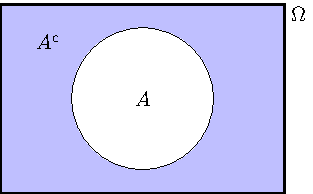
\includegraphics[width=550pt]{math1710_files/figure-latex/venn-not-1} \end{center}

\begin{center}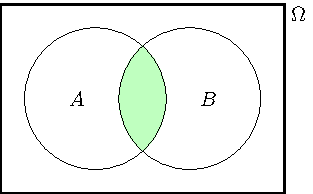
\includegraphics[width=550pt]{math1710_files/figure-latex/venn-and-1} \end{center}

\begin{center}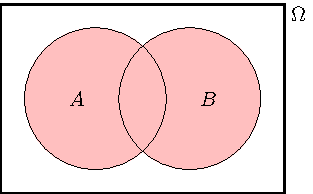
\includegraphics[width=550pt]{math1710_files/figure-latex/venn-or-1} \end{center}

\end{definition}

\begin{example}
Suppose we are rolling a dice, so our sample space is \(\Omega = \{1,2,3,4,5,6\}\). Let \(A = \{2,4,6\}\) be the event that we roll and even number, and let \(B = \{5,6\}\) be the event that we roll at least a 5. Then
\begin{align*}
A^\mathsf{c}&= \{1,3,5\} = \{\text{roll an odd number}\} ,\\
A \cap B &= \{6\} = \{\text{roll a 6}\} ,\\
A \cup B &= \{2,4,5,6\} .
\end{align*}
\end{example}

An important case is when two events \(A, B\) cannot happen at the same time; that is, \(A \cap B = \varnothing\) (``\(A\) intersect \(B\) is the empty set''). In this case, we say that \(A\) and \(B\) are \textbf{disjoint} or \textbf{mutually exclusive}. For example, when \(\Omega\) is \href{https://en.wikipedia.org/wiki/Standard_52-card_deck}{a deck of cards}, then \(A = \{\text{the card is a spade}\}\) and \(B = \{\text{the card is red}\}\) are disjoint, because a card cannot be both a spade (a black suit) and red.

You might think that if two events are disjoint, then it would be reasonable to find the probability of their union -- that is, the probability that one (and, by necessity, only one) of them happens -- you can just add the two separate probabilities together. This will be another of our ``axioms'' of probability.

There are a few rules about ways you can combine the complement, intersection and union operations. These are ways of building new events from old.

\begin{itemize}
\tightlist
\item
  The \textbf{double complement law} tells us that not-not-\(A\) is the same as \(A\):
  \[ (A^\mathsf{c})^\mathsf{c}= A .\]
  This says that if it's not ``not-raining'', then it's raining!
\item
  The \textbf{distributive laws} tells us we can ``multiply out of the brackets'' with sets:
  \begin{align*}
  A \cap (B \cup C) &= (A \cap B) \cup (A \cap C) ,\\
  A \cup (B \cap C) &= (A \cup B) \cap (A \cup C) .
  \end{align*}
  The first says that if you are eating a burger with fries or salad, then you're eating a burger with fries or eating a burger with salad. The second is a bit less intuitive, I find, but it's clear that if \(A\) is true then the first of each of the terms on the right is true, while if both \(B\) and \(C\) are true then the second of each of the terms on the right is true.
\item
  \textbf{De Morgan's laws} tell us how complements interact with intersection/unions:
  \begin{align*}
  (A \cap B)^\mathsf{c}&= A^\mathsf{c}\cup B^\mathsf{c}\\
  (A \cup B)^\mathsf{c}&= A^\mathsf{c}\cap B^\mathsf{c}
  \end{align*}
  The first of these says that if it's not a Monday in October, then either it's not Monday or it's not October (or both). The second says that if a maths lecture is not ``useful or fun'', then it's not useful and it's not fun. (\href{https://mathshistory.st-andrews.ac.uk/Biographies/De_Morgan/}{Augustus De Morgan} was a British mathematician of the 19th century who did important work in logic.)
\end{itemize}

For this module, these mostly count as ``common sense'' -- but if you ever do need to prove one of these statements (or a similar one), one way is to use a Venn diagram.

Let's prove the second distributive law,
\[   A \cup (B \cap C) = (A \cup B) \cap (A \cup C) , \]
with a Venn diagram as an example.

We can build the left-hand side of the law as:

\begin{center}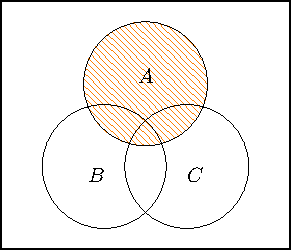
\includegraphics[width=1\linewidth]{math1710_files/figure-latex/dist1-1} \end{center}

~

\begin{center}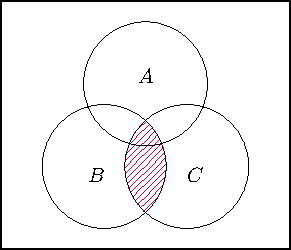
\includegraphics[width=1\linewidth]{math1710_files/figure-latex/dist2-1} \end{center}

~

\begin{center}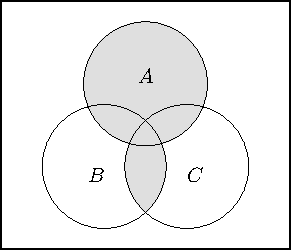
\includegraphics[width=1\linewidth]{math1710_files/figure-latex/dist3-1} \end{center}

The left-hand figure is \(\color{orange}{A}\), the middle figure is \(\color{purple}{B\cap C}\), and the right-hand figure is union of these, \(A\cup (B\cap C)\).

Then for the right-hand side of the law, we have:

\begin{center}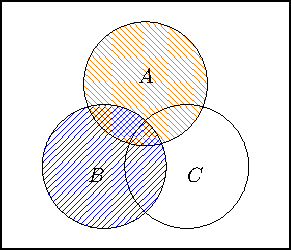
\includegraphics[width=1\linewidth]{math1710_files/figure-latex/dist4-1} \end{center}

~

\begin{center}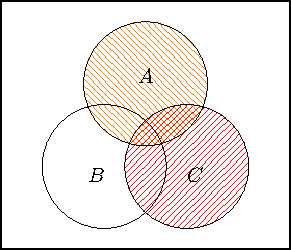
\includegraphics[width=1\linewidth]{math1710_files/figure-latex/dist5-1} \end{center}

~

\begin{center}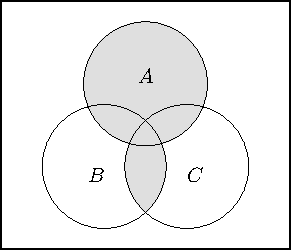
\includegraphics[width=1\linewidth]{math1710_files/figure-latex/dist6-1} \end{center}

The left-hand figure is \(\color{orange}{A} \cup \color{blue}{B}\), the middle figure is \(\color{orange}{A}\cup \color{red}{C}\), and the right-hand figure is intersection of these, \((A\cup B)\cap (A\cup C)\).

We see that the areas shaded in two right-hand figures are the same, so it is indeed the case that
\(A\cup (B\cap C) = (A\cup B)\cap (A\cup C)\).

\hypertarget{summary-L03}{%
\section*{Summary}\label{summary-L03}}
\addcontentsline{toc}{section}{Summary}

\begin{itemize}
\tightlist
\item
  A sample space \(\Omega\) is a set representing all possible sample outcomes.
\item
  An event is a subset of \(\Omega\).
\item
  For events \(A\) and \(B\), we also have the complement ``not \(A\)'' \(A^\mathsf{c}\), the intersection ``\(A\) and \(B\)'' \(A \cap B\), and the union ``\(A\) or \(B\)'' \(A \cup B\).
\end{itemize}

\textbf{Recommended reading:}

\begin{itemize}
\tightlist
\item
  \href{https://leeds.primo.exlibrisgroup.com/permalink/44LEE_INST/13rlbcs/alma991013131349705181}{Stirzaker, \emph{Elementary Probability}}, Sections 1.1 and 1.2 (plus optionally Chapter 0).
\item
  \href{https://leeds.primo.exlibrisgroup.com/permalink/44LEE_INST/13rlbcs/alma991002938669705181}{Grimmett and Welsh, \emph{Probability}}, Sections 1.1 and 1.2.
\end{itemize}

\hypertarget{L04-probability}{%
\chapter{Probability}\label{L04-probability}}

\hypertarget{axioms}{%
\section{Probability axioms}\label{axioms}}

Recall that, in this mathematics course, the probability of an event will be a real number that satisfies certain properties, which we call \textbf{axioms}.

\begin{definition}
\protect\hypertarget{def:axioms}{}\label{def:axioms}Let \(\Omega\) be a sample space. A \textbf{probability measure} on \(\Omega\) is a function \(\mathbb P\) that assigns to each event \(A \subset \Omega\) a real number \(\mathbb P(A)\), called the \textbf{probability} of \(A\), and that satisfies the following three axioms:

\begin{enumerate}
\def\labelenumi{\arabic{enumi}.}
\tightlist
\item
  \(\mathbb P(A) \geq 0\) for all events \(A \subset \Omega\);
\item
  \(\mathbb P(\Omega) = 1\);
\item
  if \(A_1, A_2, \dots\) is a finite or infinite sequence of disjoint events, then
  \[ \mathbb P(A_1 \cup A_2 \cup \cdots) = \mathbb P(A_1) + \mathbb P(A_2) + \cdots . \]
\end{enumerate}

The sample space \(\Omega\) together with the probability measure \(\mathbb P\) are called a \textbf{probability space}.
\end{definition}

Axiom 1 says that all probabilities are non-negative numbers. Axiom 2 says the probability that \emph{something} happens is 1. Axiom 3 is about \emph{disjoint} events -- recall that these are events where no two can happen at the same time, because the intersection of any pair of them is empty. {[}\emph{\textbf{Correction:} In the 3pm lecture, I wrongly said that their} union \emph{is empty.}{]} Axiom 3 says that for disjoint events the probability that one of them happens is the sum of the individual probabilities. (Those who like their mathematical statements very precise should note that an infinite sequence in Axiom 3 must be ``countable''; that is, indexed by the natural numbers \(1, 2, 3, \dots\).)

These axioms of probability (and our later results that follow from them) were first written down by the Russian mathematician \href{https://mathshistory.st-andrews.ac.uk/Biographies/Kolmogorov/}{Andrey Nikolaevich Kolmogorov} in 1933. This marked the point from when probability theory could now be considered a proper branch of mathematics -- just as legitimate as geometry or number theory -- and not just a past-time that can be useful to help gamblers calculate their odds. I always find it surprising that the axioms of probability are only 90 years old!

There are other properties that it seems natural that a probability measure should have aside from the axioms -- for example, that \(\mathbb P(A) \leq 1\) for all events \(A\). But we will show shortly that other properties can be proven just by starting from the three axioms.

But first, let's see some examples.

\begin{example}

Suppose we wish to model tossing an biased coin the is heads with probability \(p\), where \(0 \leq p \leq 1\).

Our probability space is \(\Omega = \{\text{H}, \text{T}\}\). The probability measure is given by
\begin{align*}
   \mathbb P(\varnothing) &= 0  &  \mathbb P(\{\text{H}\}) &= p \\
   \mathbb P(\{\text{T}\}) &= 1 - p  &  \mathbb P(\{\text{H},\text{T}\})  &= 1 .
\end{align*}

Let's check that the axioms hold:

\begin{enumerate}
\def\labelenumi{\arabic{enumi}.}
\tightlist
\item
  Since \(0 \leq p \leq 1\), all the probabilities are greater than or equal to 0.
\item
  It is indeed the case that \(\mathbb P(\Omega) = \mathbb P(\{\text{H},\text{T}\}) = 1\).
\item
  The only nontrivial disjoint union to check is \(\{\text{H}\} \cup \{\text{T}\} = \{\text{H},\text{T}\}\), where we see that
  \[ \mathbb P(\{\text{H}\}) + \mathbb P(\{\text{T}\}) = p + (1 - p) = 1 = \mathbb P(\{\text{H},\text{T}\}) , \]
  as required.
\end{enumerate}

\end{example}

\begin{example}
Suppose we wish to model rolling a dice.

Our sample space is \(\{1,2,3,4,5,6\}\). The probability measure is given by
\[ \mathbb P(A) = \frac{|A|}{6} , \]
where \(|A|\) is the number of sample outcomes in \(A\).

So, for example, the probability of rolling an even number is
\[ \mathbb P(\{2,4,6\}) = \frac36 = \frac12 . \]
\end{example}

The dice rolling is a particular case of the ``classical probability'' of equally likely outcomes. We'll look at this more in the next lecture, and prove that the classical probability measure does indeed satisfy the axioms

\hypertarget{prob-properties}{%
\section{Properties of probability}\label{prob-properties}}

The axioms of Definition \ref{def:axioms} only gave us some of the properties that we would like a probability measure to have. Our task now (in this subsection and the next) is to carefully prove how these other properties follow from just those axioms. In particular, we're not allowed to make claims that merely ``seem likely to be true'' or ``are common sense'' -- we can only use the three axioms together with strict logical deductions and nothing else.

\begin{theorem}

Let \(\Omega\) be a sample space with a probability measure \(\mathbb P\). Then we have the following:

\begin{enumerate}
\def\labelenumi{\arabic{enumi}.}
\tightlist
\item
  \(\mathbb P(\varnothing) = 0\).
\item
  \(\mathbb P(A^\mathsf{c}) = 1 - \mathbb P(A)\) for all events \(A \subset \Omega\).
\item
  For events \(A\) and \(B\) with \(B \subset A\), we have \(\mathbb P(B) \leq \mathbb P(A)\).
\item
  \(0 \leq \mathbb P(A) \leq 1\) for all events \(A \subset \Omega\).
\end{enumerate}

\end{theorem}

Importantly, the second result here tells us how to deal with complements or ``not'' events: the probability of \(A\) \emph{not} happening is 1 minus the probability it does happen. This is often very useful.

\begin{proof}
The key with most of these ``prove from the axioms'' problems is to think of a way to write the relevant events as part of a \emph{disjoint} union, then use Axiom 3. Statements 1 and 2 are exercises for you on \protect\hyperlink{P2}{Problem Sheet 2}. We'll start with the third statement.

Here, since \(B\) is a subset of \(A\), meaning that \(B\) is entirely inside \(A\).

\begin{center}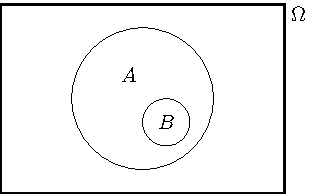
\includegraphics[width=320pt]{math1710_files/figure-latex/subs0-1} \end{center}

It would be useful to write \(A\) as a \emph{disjoint} union of \(\color{orange}B\) and {``the bit of \(A\) that isn't in \(B\)''}. That is, we have the disjoint union
\[ A = \color{orange}B \cup (\color{purple}{A \cap B^\mathsf{c}}) .\]

\begin{center}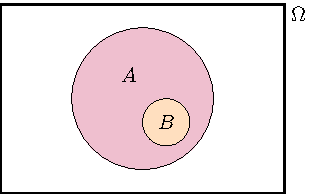
\includegraphics[width=320pt]{math1710_files/figure-latex/subs-1} \end{center}

Applying Axiom 3 to this disjoint union gives
\[ \mathbb P(A) =  \mathbb P(\color{orange}B) + \mathbb P(\color{purple}{A \cap B^\mathsf{c}}) . \]

We're happy to see the term on the left-hand side and the first term on the right-hand side. But what about the awkward \(\mathbb P(A \cap B^\mathsf{c})\)? Well, by Axiom 1, we know that the probability of any event is greater than or equal to 0, so in particular. \(\mathbb P(A \cap B^\mathsf{c}) \geq 0\). Hence
\[ \mathbb P(A)  \geq \mathbb P(B) + 0 = \mathbb P(B) , \]
and we are done with the third statement.

For the fourth statement, we have \(\mathbb P(A) \geq 0\) directly from Axiom 1, so only need to show that \(\mathbb P(A) \leq 1\). We can do this using the third statement of this theorem. For any event \(A\) we have \(A \subset \Omega\), so the third statement tells us that \(\mathbb P(A) \leq \mathbb P(\Omega)\). But Axiom 2 tells us that \(\mathbb P(\Omega) = 1\), so \(\mathbb P(A) \leq 1\) and we are done.
\end{proof}

\hypertarget{addition}{%
\section{Addition rules for unions}\label{addition}}

If we have two or more events, we'd like to work out the probability of their union; that is, the probability that at least one of them occurs.

We already have an addition rule for \emph{disjoint} unions.

\begin{theorem}
Let \(A, B \subset \Omega\) be two disjoint events. Then
\[ \mathbb P(A \cup B) = \mathbb P(A) + \mathbb P(B) . \]
\end{theorem}

\begin{proof}
In Axiom 3, take the finite sequence \(A_1 = A\), \(A_2 = B\).
\end{proof}

But what about if \(A\) and \(B\) are not disjoint? Then we have the following.

\begin{theorem}
Let \(A, B \subset \Omega\) be two events. Then
\[ \mathbb P(A \cup B) = \mathbb P(A) + \mathbb P(B) - \mathbb P(A \cap B) . \]
\end{theorem}

You may have seen this result before. You've perhaps justified it by saying something like this: ``We can add the two probabilities together, except now we've double-counted the overlap, so we have to take the probability of that away.'' Maybe you drew a Venn diagram. That's OK as a way to remember the result -- but this is a proper university mathematics course, so we have to carefully \emph{prove} it starting from just the axioms and nothing else.

\begin{proof}
The problem here is that \(A\) and \(B\) are not (in general) disjoint, so we can't apply Axiom 3.

\begin{center}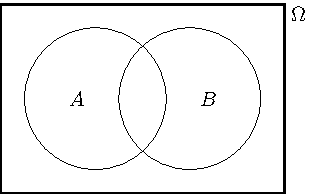
\includegraphics[width=320pt]{math1710_files/figure-latex/add3-1} \end{center}

Instead, let's split this up into the three disjoint bits: {``\(A\) but not \(B\)''} \(\color{red}{A \cap B^\mathsf{c}}\), {``\(B\) but not \(A\)''} \(\color{blue}{B \cap A^\mathsf{c}}\), and {``both''} \(\color{green}{A \cap B}\).

\begin{center}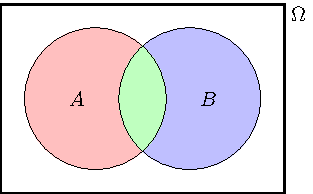
\includegraphics[width=320pt]{math1710_files/figure-latex/add4-1} \end{center}

Now we can write \(A\), \(B\) and \(A \cup B\) in terms of these disjoint bits.
\begin{align}
A &= (\color{red}{A \cap B^\mathsf{c}}) \cup (\color{green}{A \cap B}) \\
B &= (\color{blue}{B \cap A^\mathsf{c}}) \cup (\color{green}{A \cap B}) \\
A \cup B &= (\color{red}{A \cap B^\mathsf{c}}) \cup (\color{blue}{B \cap A^\mathsf{c}}) \cup (\color{green}{A \cap B}),
\end{align}
with all the unions on the right-hand side being disjoint. Applying Axiom 3 to them all gives
\begin{align}
\mathbb P(A) &= \mathbb P(\color{red}{A \cap B^\mathsf{c}}) + \mathbb P(\color{green}{A \cap B}) \label{eq:un1}  \\
\mathbb P(B) &= \mathbb P(\color{blue}{B \cap A^\mathsf{c}}) + \mathbb P(\color{green}{A \cap B})  \label{eq:un2} \\
\mathbb P(A \cup B) &= \mathbb P(\color{red}{A \cap B^\mathsf{c}}) + \mathbb P(\color{blue}{B \cap A^\mathsf{c}}) + \mathbb P(\color{green}{A \cap B}) . \label{eq:un3}
\end{align}
Here, \eqref{eq:un3} is looking good, but we need to get rid of the awkward \(\mathbb P(\color{red}{A \cap B^\mathsf{c}})\) and \(\mathbb P(\color{blue}{B \cap A^\mathsf{c}})\) terms. We can do that be rearranging \eqref{eq:un1} and \eqref{eq:un2} to get
\begin{align}
\mathbb P(\color{red}{A \cap B^\mathsf{c}}) &= \mathbb P(A) - \mathbb P(\color{green}{A \cap B}) \\
\mathbb P(\color{blue}{B \cap A^\mathsf{c}}) &= \mathbb P(B) - \mathbb P(\color{green}{A \cap B}) .
\end{align}
Substituting these into \eqref{eq:un3} gives
\begin{align}
\mathbb P(A \cup B) &= \mathbb P(A) - \mathbb P(\color{green}{A \cap B}) + \mathbb P(B) - \mathbb P(\color{green}{A \cap B}) + \mathbb P(\color{green}{A \cap B}) \\
  &= \mathbb P(A)+ \mathbb P(B) - \mathbb P(A \cap B) ,
\end{align}
as required.
\end{proof}

\begin{example}
\emph{Consider picking a card from a \href{https://en.wikipedia.org/wiki/Standard_52-card_deck}{standard 52-card deck} at random, with \(\mathbb P(A) = |A|/52\). What's the probability the card is a spade or an ace?}

It is possible to just to work this out directly. But let's use our addition law for unions.

We have \(\mathbb P(\text{spade}) = \frac{13}{52}\) and \(\mathbb P(\text{ace}) = \frac{4}{52}\). So we have
\[ \mathbb P(\text{spade or ace}) = \tfrac{13}{52} + \tfrac{4}{52} - \mathbb P(\text{spade and ace}) . \]
But \(\mathbb P(\text{spade and ace})\) is the probability of picking the ace of spades, which is \(\frac{1}{52}\). Therefore
\[ \mathbb P(\text{spade or ace}) = \tfrac{13}{52} + \tfrac{4}{52}  - \tfrac{1}{52} = \tfrac{16}{52} = \tfrac{4}{13} . \]
\end{example}

\hypertarget{summary-L04}{%
\section*{Summary}\label{summary-L04}}
\addcontentsline{toc}{section}{Summary}

\begin{itemize}
\tightlist
\item
  The axioms of probability are (1) \(\mathbb P(A) \geq 0\); (2) \(\mathbb P(\Omega) = 1\); and (3) that for disjoint events \(A_1, A_2, \dots\), we have \(\mathbb P(A_1 \cup A_2 \cup \cdots) = \mathbb P(A_1) + \mathbb P(A_2) + \cdots\).
\item
  Other properties can be proven from these axioms, like the complement rule \(\mathbb P(A^\mathsf{c}) = 1 - \mathbb P(A)\), and the addition rule for unions \(\mathbb P(A \cup B) = \mathbb P(A) + \mathbb P(B) - \mathbb P(A \cap B)\).
\end{itemize}

\textbf{Recommended reading:}

\begin{itemize}
\tightlist
\item
  \href{https://leeds.primo.exlibrisgroup.com/permalink/44LEE_INST/13rlbcs/alma991013131349705181}{Stirzaker, \emph{Elementary Probability}}, Sections 1.3 and 1.4.
\item
  \href{https://leeds.primo.exlibrisgroup.com/permalink/44LEE_INST/13rlbcs/alma991002938669705181}{Grimmett and Welsh, \emph{Probability}}, Sections 1.3 and 1.4.
\end{itemize}

On \protect\hyperlink{P2}{Problem Sheet 2}, you should now be able to complete Questions A1, A2, B1, B2 and perhaps C1.

\hypertarget{L05-classical-i}{%
\chapter{Classical probability I}\label{L05-classical-i}}

\hypertarget{summary-L05}{%
\section*{Summary}\label{summary-L05}}
\addcontentsline{toc}{section}{Summary}

\begin{itemize}
\tightlist
\item
  ``Classical probability'' describes the situation where there are finitely many equally likely outcomes. The classical probability \(\mathbb P(A) = |A|/|\Omega|\) requires us to count how many outcomes there are in events or sample spaces.
\item
  The multiplication principle says that \(n\) choices followed by \(m\) choices makes \(n \times m\) choices in total.
\item
  Sampling \(k\) objects out of \(n\) with replacement gives \(n^k\) choices.
\item
  Sampling \(k\) objects out of \(n\) without replacement gives \(n^{\underline{k}} = n(n-1)\cdots(n-k+1)\) choices.
\end{itemize}

\textbf{Recommended reading:}

\begin{itemize}
\tightlist
\item
  \href{https://leeds.primo.exlibrisgroup.com/permalink/44LEE_INST/13rlbcs/alma991013131349705181}{Stirzaker, \emph{Elementary Probability}}, Sections 3.1 and 3.2.
\end{itemize}

\hypertarget{L06-classical-ii}{%
\chapter{Classical probability II}\label{L06-classical-ii}}

\hypertarget{summary-L06}{%
\section*{Summary}\label{summary-L06}}
\addcontentsline{toc}{section}{Summary}

\begin{itemize}
\tightlist
\item
  Ordering \(n\) objects can be done in \(n! = n^{\underline{n}} = n(n-1)\cdots2\cdot1\) ways.
\item
  The number of ways to sample \(k\) objects out of \(n\) when the order doesn't matter is given by the binomial coefficient \(\binom nk = {n}^{\underline{k}}/k!\).
\end{itemize}

\textbf{Recommended reading:}

\begin{itemize}
\tightlist
\item
  \href{https://leeds.primo.exlibrisgroup.com/permalink/44LEE_INST/13rlbcs/alma991013131349705181}{Stirzaker, \emph{Elementary Probability}}, Sections 3.2 and 3.3.
\end{itemize}

On \protect\hyperlink{P2}{Problem Sheet 2}, you should now be able to complete all questions.

\hypertarget{P2}{%
\chapter*{Problem Sheet 2}\label{P2}}
\addcontentsline{toc}{chapter}{Problem Sheet 2}

\commfalse

This is Problem Sheet 2. This problem sheet covers material from Lectures 3 to 6. You should work through all the questions on this problem sheet in preparation for your tutorial in Week 4. The problem sheet contains two assessed questions, which are due in by \textbf{2pm on Monday 30 October}.

\hypertarget{P2-short}{%
\section*{A: Short questions}\label{P2-short}}
\addcontentsline{toc}{section}{A: Short questions}

\textbf{A1.} Suppose you toss a coin 4 times.

\textbf{(a)} What would you suggest for a sample space \(\Omega\) \textbf{(i)} if you only care about the total number of heads; \textbf{(ii)} if you care about the result of each coin toss?

\textbf{(b)} For each of the cases in part (a), what is \(|\Omega|\)?

\begin{myanswers}
\emph{Solution.}

\textbf{(i)} We can take \(\Omega = \{0,1,2,3,4\}\), with \(|\Omega| = 5\).

\textbf{(ii)} Here, \(\Omega = \{ \text{HHHH}, \text{HHHT}, \text{HHTH},\dots, \text{TTTT} \}\) should be the set of all sequences of four ``H''s or ``T''s. So here, \(|\Omega| = 2^4 = 16\).

\end{myanswers}

\textbf{A2.} Let \(A\), \(B\) and \(C\) be events in a sample space \(\Omega\). Write the following events using only \(A\), \(B\), \(C\) and the complement, intersection, and union operations.

\textbf{(a)} \(C\) happens but \(A\) doesn't.

\begin{myanswers}
\emph{Solution.} This is ``\(C\) and not \(A\)'': \(C\cap A^{\mathsf{c}}\).

\end{myanswers}

\textbf{(b)} At least one of \(A\), \(B\) and \(C\) happens.

\begin{myanswers}
\emph{Solution.} This is simply the union \(A \cup B\cup C\).

\end{myanswers}

\textbf{(c)} Exactly one of \(B\) or \(C\) happens.

\begin{myanswers}
\emph{Solution.} One way to write this is to split it up as ``\,`\(B\) but not \(C\)' or `\(C\) but not \(B\)'\,'', which is \((B \cap C^{\mathsf{c}}) \cup (B^{\mathsf{c}} \cap C)\).

An alternative is to split it up as ``\,`\(B\) or \(C\)' but not `both \(B\) and \(C\)'\,'', which is \((B \cup C) \cap (B\cap C)^{\mathsf{c}}\).

You can check these are equal by (for example) using De Morgan's law and the distributive law to expand out the second version.

\end{myanswers}

\textbf{(d)} Exactly two of \(A\), \(B\) and \(C\) happens.

\begin{myanswers}
\emph{Solution.} I would split this up into ``\(A\) and \(B\) but not \(C\)'', ``\(A\) and \(C\) but not \(B\)'', and ``\(B\) and \(C\) but not \(A\)'' and take the union. This gives
\[  (A \cap B \cap C^{\mathsf{c}}) \cup (A \cap B^{\mathsf{c}} \cap C) \cup (A^{\mathsf{c}} \cap B \cap C) . \]
There are other equivalent formulations.

\end{myanswers}

\textbf{A3.} What is the value of the following expressions?

\textbf{(a)} \(6!\)

\begin{myanswers}
\emph{Solution.}
\[ 6! = 6 \times 5 \times 4 \times 3 \times 2 \times 1 = 720. \]

\end{myanswers}

\textbf{(b)} \(8^4\)

\begin{myanswers}
\emph{Solution.}
\[ 8^4 = 8 \times 8 \times 8 \times 8 = 4096 \]

\end{myanswers}

\textbf{(c)} \({8}^{\underline{4}}\)

\begin{myanswers}
\emph{Solution.}
\[ {8}^{\underline{4}} = 8 \times 7 \times 6 \times 5 = 1680 \]

\end{myanswers}

\textbf{(d)} \({\displaystyle \binom{10}{4}}\)

\begin{myanswers}
\emph{Solution.}
\[ \binom{10}{4} = \frac{10 \times 9 \times 8 \times 7}{4\times 3\times 2\times 1} = 210 \]

\end{myanswers}

\textbf{A4.} An urn contains 4 red balls and 6 blue balls. Two balls are drawn from the urn. What is the probability that both balls are red, if the balls are drawn \textbf{(a)} with replacement; \textbf{(b)} without replacement?

\begin{myanswers}
\emph{Solution.}

\textbf{(a)} There are \(|\Omega| = 10^2 = 100\) ways to draw two balls with replacement. There are \(|A| = 4^2=16\) ways to draw two blue balls. So
\(\mathbb P(A) = \frac{16}{100} = 0.16\).

\textbf{(b)} There are \(|\Omega| = {10}^{\underline{2}} = 10 \times 9 = 90\) ways to draw two balls without replacement. There are \(|A| = {4}^{\underline{2}} = 4 \times 3 = 12\) to draw two blue balls. So
\(\mathbb P(A) = \frac{12}{90} = \frac{2}{15} = 0.133\).

\end{myanswers}

\hypertarget{P2-long}{%
\section*{B: Long questions}\label{P2-long}}
\addcontentsline{toc}{section}{B: Long questions}

\textbf{B1.} Starting from just the three probability axioms, prove the following statements:

\textbf{(a)} \(\mathbb P(\varnothing) = 0\).

\begin{myanswers}
\emph{Solution.} Let \(A\) be any event (such as \(A = \varnothing\) or \(A = \Omega\), for example). Then \(A \cup \varnothing = A\), and the union is disjoint -- since \(\varnothing\) contains no sample points, it certainly can't contain any sample points that are also in \(A\). Then applying Axiom 3, we get \(\mathbb P(A) + \mathbb P(\varnothing) = \mathbb P(A)\). Subtracting \(\mathbb P(A)\) from both sides gives the result.

\emph{Alternatively}, if you prove part (b) first, you can apply that with \(A = \varnothing\). Since \(\varnothing^\mathsf{c}= \Omega\) and Axiom 2 tells us that \(\mathbb P(\Omega) = 1\), the result follows.

\textbf{Group feedback:} With this, and most ``prove from the axioms'' questions, the key is to find a relevant disjoint union, which then allows us to use Axiom 3. So if we can find \(C = A \cup B\) as a disjoint union (hopefully containing some events relevant to the question at hand), Axiom 3 allows us to write \(\mathbb P(C) = \mathbb P(A) + \mathbb P(B)\).

\end{myanswers}

\textbf{(b)} \(\mathbb P(A^\mathsf{c}) = 1 - \mathbb P(A)\).

\begin{myanswers}
\emph{Solution.} A very useful and relevant disjoint union is \(A \cup A^\mathsf{c}= \Omega\). Applying Axiom 3 gives us \(\mathbb P(A) + \mathbb P(A^\mathsf{c}) = \mathbb P(\Omega)\). But Axiom 2 tells us that \(\mathbb P(\Omega) = 1\), so \(\mathbb P(A) + \mathbb P(A^\mathsf{c}) = 1\). Rearranging gives the result.

\end{myanswers}

\textbf{B2.} In this question, you will have to use the standard two-event form of the addition rule for unions
\[ \mathbb P(A \cup B) = \mathbb P(A) + \mathbb P(B) - \mathbb P(A \cap B) . \]

\textbf{(a)} Using the two-event addition rule, show that
\[ \mathbb P(C \cup D \cup E) = \mathbb P(C) + \mathbb P(D \cup E) - \mathbb P\big(C \cap (D \cup E)\big).  \]

\begin{myanswers}
\emph{Solution.} As with the Cauchy--Schwarz question from Problem Sheet 1, the key is to make a good choice for what \(A\) and \(B\) should be. This time, \(A = C\) and \(B = D \cup E\) will work well, since \(C \cup (D \cup E) = C \cup D \cup E\). (You can call this ``associativity'', if you like.) Making that substitution immediately gives us
\[ \mathbb P(C \cup D \cup E) = \mathbb P(C) + \mathbb P(D \cup E) - \mathbb P\big(C \cap (D \cup E)\big) ,  \]
as required.

\end{myanswers}

\textbf{(b)} Using your result from part (a), the two-event addition rule, the distributive law, and the two-event addition rule again, prove the three-event form of the addition rule for unions:
\[
  \mathbb P(C \cup D \cup E) = \mathbb P(C) + \mathbb P(D) + \mathbb P(E) 
  - \mathbb P(C \cap D) - \mathbb P(C \cap E) - \mathbb P(D \cap E) + \mathbb P(C \cap D \cap E) .
\]

\begin{myanswers}
\emph{Solution.}
Let's take the three terms on the right of the equation from part (a) separately.

The first term is \(\mathbb P(C)\), which is fine as it is.

The second term is \(\mathbb P(D \cup E)\). This is the probability of the union of two events, so we can use addition rule for the union of two events to get
\[ \mathbb P(D \cup E) = \mathbb P(D) + \mathbb P(E) - \mathbb P(D \cap E) . \]

The third term is \(\mathbb P\big(C \cap (D \cup E)\big)\). If we use the distributive law, as suggested in the question, we get \(C \cap (D \cup E) = (C \cap D) \cup (C\cap E)\), so we want to find \(\mathbb P\big((C \cap D) \cup (C\cap E)\big)\). But this is another union of two events again, this time with \(A = C \cap D\) and \(B = C \cap E\). So the two-event addition rule gives
\[ \mathbb P\big((C \cap D) \cup (C\cap E)\big) = \mathbb P(C \cap D) + \mathbb P(C \cap E) - \mathbb P(C \cap D \cap E) , \]
since \((C \cap D) \cap (C \cap E) = C \cap D \cap E\).

Finally, we put this all together, and get
\begin{align*}
  \mathbb P(C &\cup D \cup E) \\
  &= \mathbb P(C) + \big(\mathbb P(D) + \mathbb P(E) - \mathbb P(D \cap E)\big) - \big(\mathbb P(C \cap D) + \mathbb P(C \cap E) - \mathbb P(C \cap D \cap E)\big) \\
  &= \mathbb P(C) + \mathbb P(D) + \mathbb P(E) - \mathbb P(C \cap D) - \mathbb P(C \cap E) - \mathbb P(D \cap E) + \mathbb P(C \cap D \cap E) , 
\end{align*}
which is what we wanted.

\end{myanswers}

\textbf{B3.} Suppose we pick a number at random from the set \(\{1, 2, \dots, 2023\}\).

\textbf{(a)} What is the probability that the number is divisible by 5?

\begin{myanswers}

\emph{Solution.} The sample space is \(\Omega = \{1, 2, \dots, 2023\}\). Clearly \(|\Omega| = 2023\). The event in question is \(A = \{5, 10, \dots, 2020\}\) of numbers up to 2022 that are divisible by 5. Thus \(|A|\) is the largest integer no bigger than \(\frac{2023}{5} = 404.6\), which is 404, as this is how many times 5 ``goes into'' 2022. Hence
\[ \mathbb P(A) = \frac{|A|}{|\Omega|} = \frac{404}{2023} = 0.1997 , \]
just a tiny bit smaller than \(\frac{1}{5}\).

\textbf{Group feedback:} With these ``classical probability'' questions, the steps should always be:

\begin{enumerate}
\def\labelenumi{\arabic{enumi}.}
\tightlist
\item
  State clearly what the sample space \(\Omega\) is.
\item
  Count how many outcomes \(|\Omega|\) are in the sample space.
\item
  State clearly what the event \(A\) is.
\item
  Count how many outcomes \(|A|\) are in the event.
\item
  The desired probability is then \(\mathbb P(A) = |A|/|\Omega|\).
\end{enumerate}

\end{myanswers}

\textbf{(b)} What is the probability the number is divisible by 5 or by 7?

\begin{myanswers}
\emph{Solution.} With the same \(\Omega\) and \(A\), now let \(B\) be the numbers up to 2023 divisible by \(7\); so we're looking for \(\mathbb P(A \cup B)\). By the addition rule for unions, this is
\[ \mathbb P(A \cup B) = \mathbb P(A) + \mathbb P(B) - \mathbb P(A \cap B) . \]
We already know \(\mathbb P(A) = \frac{404}{2022}\), so need to find out \(\mathbb P(B)\) and \(\mathbb P(A \cap B)\).

This time, 7 goes into 2023 exactly, so \(|B|\) is \(\frac{2023}{7} = 289\). So
\[ \mathbb P(B) = \frac{|B|}{|\Omega|} = \frac{289}{2023} = \frac{1}{7}  . \]

Now, \(A \cap B\) is the set of numbers divisible by both 5 and 7, which is precisely the numbers divisible by their least common multiple \(5 \times 7 = 35\). Then \(|A \cap B|\) is \(\frac{2023}{35} = 57.8\) rounded down, so \(\mathbb P(A \cap B) = \frac{57}{2023}\).

So finally, we have
\[ \mathbb P(A \cup B) = \frac{404}{2023} + \frac{289}{2023} - \frac{57}{2023} = \frac{636}{2023} = 0.314 , \]
just a tiny bit larger than \(\frac{11}{35}\)

\end{myanswers}

\textbf{B4.} Eight friends are about to sit down at random at a round table. Find the probability that

\textbf{(a)} Ashley and Brook sit next to each other, with Chris directly opposite Brook;

\begin{myanswers}
\emph{Solution.}
Let \(\Omega\) be the sample space of ways the friends can sit around the table. This is an ordering problem, so \(|\Omega| = 8!\).

Let \(A\) be the event in the question. What is \(|A|\)? Well,

\begin{itemize}
\tightlist
\item
  Ashley can sit anywhere, so has 8 choices of seat.
\item
  Brook can sit either directly to Ashley's left or directly to Ashley's right, so has 2 choices of seat.
\item
  Chris must sit directly opposite Brook, so only has 1 choice of seat.
\item
  The remaining five friends can fill up the remaining seats however they like, so have 5, 4, 3, 2, and 1 choices respectively.
\end{itemize}

Hence \(|A| = 8 \times 2 \times 1 \times 5 \times 4 \times 3 \times 2 \times 1\). Thus we get
\[ \mathbb P(A) = \frac{|A|}{|\Omega|} = \frac{8 \times 2 \times 1 \times 5 \times 4 \times 3 \times 2 \times 1}{8 \times 7 \times 6 \times 5 \times 4 \times 3 \times 2 \times 1} = \frac{2 \times 1}{7 \times 6} = \frac{1}{21} . \]

\textbf{Group feedback:} As we have discussed more recently, after this Problem Sheet was assigned, often ``classical probability'' problems also can be equivalently solved by the step-by-step ``chain rule'' method. Can you use a chain rule argument to find the same answer as
\[ \mathbb P(A) = 1 \times \frac27 \times \frac16 \times 1 \times 1 \times 1 \times 1 \times 1 = \frac{1}{21} ? \]

\end{myanswers}

\textbf{(b)} neither Ashley, Brook nor Chris sit next to each other.

\begin{myanswers}
\emph{Solution.}
The sample space \(\Omega\) is as before. Let's count the outcomes in \(B\), the event in the question.

\begin{itemize}
\tightlist
\item
  Ashley can sit anywhere, so has 8 choices of seat.
\item
  Chris's number of choices will depend on where Brook sits, so we'll have to count Brook's and Chris's choices together:

  \begin{itemize}
  \tightlist
  \item
    Brook cannot sit next to Ashley.
  \item
    If Brook sits next-but-one to Ashley -- of which there are 2 choices -- then Chris has 3 choices: Chris cannot sit on the seat directly between Ashley and Brook, nor directly next to Ashley on the other side, nor directly next to Brook on the other side, leaving \(6-3=3\) choices.
  \item
    If Brook sits neither next nor next-but-one to Ashley -- of which there are 3 choices -- then Chris has 2 choices: he cannot sit to the right or left of Ashley, nor to the right or left of Brook, leaving \(6-4=2\) choices.
  \end{itemize}
\item
  The remaining friends have 5, 4, 3, 2, and 1 choices again.
\end{itemize}

Hence, \(|B| = 8 \times (2\times 3 + 3 \times 2) \times 5 \times 4 \times 3 \times 2 \times 1\). So
\[ \mathbb P(B) = \frac{|B|}{|\Omega|} = \frac{8 \times (2\times 3 + 3 \times 2) \times 5 \times 4 \times 3 \times 2 \times 1}{8 \times 7 \times 6 \times 5 \times 4 \times 3 \times 2 \times 1} = \frac{2\times 3 + 3 \times 2}{7 \times 6} = \frac{12}{42} = \frac{2}{7} .  \]

\emph{Alternatively}, in a previous year's tutorial, a MATH1710 student suggested to me the following rather elegant solution. Suppose the five other friends are already sat at a round table with five chairs. Ashley, then Brook, then Chris will each bring along their own chair, and push into one of the gaps between the friends.

Ashley has 5 gaps to choose from, then Brook will have 6 gaps (Ashley joining the table will have increased the number of gaps by 1), then Chris will have 7, so the total number of ways they can push in is \(|\Omega| = 5 \times 6 \times 7\).

To not sit next to each other, Ashley can push in any of the 5 gaps, Brook only has \(6 - 2 = 4\) choices (not in the gap directly to the left or right of Ashley), and Chris only has \(7 - 4 = 3\) choices (not in the gaps directly to the left or right of Ashley nor the gaps directly to the left or right of Brook -- these four gaps are distinct assuming Brook was not next to Ashley). Hence \(|B| = 5 \times 4 \times 3\), and we have
\[ \mathbb P(B) = \frac{5 \times 4 \times 3}{5 \times 6 \times 7} = \frac{4 \times 3}{6 \times 7} = \frac{12}{42} = \frac{2}{7}.  \]

\textbf{Group feedback:} Again, an equivalent answer can be derived using the step-by-step ``chain rule'' method.

\end{myanswers}

\textbf{B5.} A ``random digit'' is a number chosen at random from \(\{0, 1, \dots, 9\}\), each with equal probability. A statistician chooses \(n\) random digits (with replacement).

\textbf{(a)} For \(k = 0, 1, \dots, 9\), let \(A_k\) be the event that all the digits are \(k\) or smaller. What is the probability of \(A_k\), as a function of \(k\) and \(n\)?

\begin{myanswers}
\emph{Solution.}
The sample space is \(\Omega = \{0,1,\dots,9\}^n\), the set of length-\(n\) sequences of digits between \(0\) and \(9\). The number of these is \(|\Omega| = 10^n\), as there are 10 choices for each of the \(n\) digits.

The event \(A_k\) is \(\{0,1,\dots,k\}^n\), the set of length-\(n\) sequences of digits that are between \(0\) and \(k\). The number of these is \(|A_k| = (k+1)^n\). (Note that it's \(k+1\) because we're allowing 0 as well.)

Hence, the probability is
\[ \mathbb P(A_k) = \frac{|A_k|}{|\Omega|} = \frac{(k+1)^n}{10^n} . \]

\end{myanswers}

\textbf{(b)} Let \(B_k\) be the event that the largest digit chosen is equal to \(k\). By finding a relationship between \(B_k\), \(A_{k-1}\) and \(A_k\), or otherwise, show that
\[ \mathbb P(B_k) = \frac{(k+1)^n - k^n}{10^n} . \]

\begin{myanswers}
\emph{Solution.}
Consider the event \(A_k\) that all the digits are at most \(k\). Within \(A_k\), \emph{either} one or more of the digits equal \(k\), in which case that \(k\) is the largest digit and we are in \(B_k\); \emph{or} none of the digits equal \(k\), in which case they are all at most \(k-1\), and we are in \(A_{k-1}\). Only one of these two possibilitie can occur, so we have a disjoint union
\[ A_k = B_k \cup A_{k-1} . \]

Applying Axiom 3 to the disjoint union gives
\[ \mathbb P(A_k) = \mathbb P(B_k) + \mathbb P(A_{k-1}) . \]
Rearranging this gives
\[ \mathbb P(B_k) = \mathbb P(A_k) - \mathbb P(A_{k-1}) . \]
Substituting in the answer from part (a) gives
\[\mathbb P(B_k) = \frac{(k+1)^n}{10^n} - \frac{(k-1+1)^n}{10^n} = \frac{(k+1)^n - k^n}{10^n} . \]

\end{myanswers}

\hypertarget{P2-assessed}{%
\section*{C: Assessed questions}\label{P2-assessed}}
\addcontentsline{toc}{section}{C: Assessed questions}

The last two questions are \textbf{assessed questions}. These two questions count for 3\% of your final mark for this module.

The deadline for submitting your solutions is \textbf{2pm on Monday 30 October} at the beginning of Week 5. You should submit a PDF to Gradescope.
Your work will be marked by your tutor and returned on Monday 6 November, when solutions will also be made available.

Both questions are ``long questions'', where the marks are not only for mathematical accuracy but also for the clarity and completeness of your explanatory writing.

You should not collaborate with others on the assessed questions: your answers must represent solely your own work. The University's rules on \href{https://library.leeds.ac.uk/info/1401/academic_skills/46/academic_integrity_and_plagiarism}{academic integrity} -- and the related punishments for violating them -- apply to your work on the assessed questions.

\textbf{C1.} Let \(\Omega\) be a sample space with a probability measure \(\mathbb P\), and let \(A, B \subset \Omega\) be events. For each of the following statements, state whether the statement is true or false (that is, always true or sometimes false). If it is true, briefly justify the statement; if it is false, give a counterexample.

\textbf{(a)} If \(\mathbb P(A) \leq \mathbb P(B)\), then \(A \subset B\).

\begin{myanswers}
\emph{Hint.} Try to find a counterexample. Make sure you're paying attention to the direction of implication (the other direction is true).


\end{myanswers}

\textbf{(b)} \(\mathbb P(A \cap B) + \mathbb P(A \cap B^{\mathsf{c}}) = \mathbb P(A)\).

\begin{myanswers}
\emph{Hint.} Is there a relevant disjoint union here?


\end{myanswers}

\textbf{(c)} \(\mathbb P(A \cup B) \leq \mathbb P(A)\)

\begin{myanswers}
\emph{Hint.} You'd expect the inequality to be the other way round -- so it should be possible to find a counterexample.

\end{myanswers}

\textbf{(d)} If \(A\) and \(B\) are disjoint, then \(\mathbb P((A \cup B)^{\mathsf{c}}) = 1 - \mathbb P(A) - \mathbb P(B)\).

\begin{myanswers}
\emph{Hint.} Can you use the complement rule to start off with?

\end{myanswers}

\textbf{C2.} An urn contains 15 balls: 4 red balls, 5 blue balls, and 6 green balls.

\textbf{(a)} If three balls are drawn \emph{with} replacement, what is the probability that all three balls are the \emph{same} colour?

\begin{myanswers}
\emph{Hint.} If \(A\) is the event all three balls are the same colour, then we have a disjoint union \(A = A_{\text{red}} \cup A_{\text{blue}} \cup A_{\text{green}}\), where \(A_{\text{red}}\) is the event all three balls are red, and so on.

\end{myanswers}

\textbf{(b)} If three balls are drawn \emph{without} replacement, what is the probability that all three balls are \emph{different} colours?

\begin{myanswers}
\emph{Hint.} One way to do this is to look at the ordered collection of balls, and look at all \(3!\) possible orderings red-blue-green, red-green-blue, etc.

Another way is to look at the unordered collection, so the denominator is \(\binom{15}{3}\).

\end{myanswers}

\hypertarget{P2-short-sols}{%
\section*{Solutions to short questions}\label{P2-short-sols}}
\addcontentsline{toc}{section}{Solutions to short questions}

\textbf{A1.} (a) (i) \(\{0,1,\dots, 4\}\) (ii) \(\{ \text{HHHH}, \text{HHHT}, \text{HHTH},\dots, \text{TTTT} \}\) (b) (i) 5 (ii) 16.\\
\textbf{A2.} (a) \(C \cap A^\mathsf{c}\) (b) \(A \cup B \cup C\) (c) \((B \cup C) \cap (B \cap C)^\mathsf{c}\) or \((B \cap C^\mathsf{c}) \cup (B^\mathsf{c}\cap C)\)\\
(d) \((A \cap B \cap C^\mathsf{c}) \cup (A \cap B^\mathsf{c}\cap C) \cup (A^\mathsf{c}\cap B \cap C)\) or other equivalent\\
\textbf{A3.} (a) 720 (b) 4092 (c) 1680 (d) 210\\
\textbf{A4.} (a) \(\frac{4}{25} = 0.16\) (b) \(\frac{2}{15} = 0.133\)

\hypertarget{part-other-stuff}{%
\part*{Other stuff}\label{part-other-stuff}}
\addcontentsline{toc}{part}{Other stuff}

\hypertarget{R}{%
\chapter*{R Worksheets}\label{R}}
\addcontentsline{toc}{chapter}{R Worksheets}

Each week (starting in Week 2) there will be an R worksheet to work through in your own time. I recommend spending about one hour on each worksheet, plus one extra hour for even-numbered worksheets with assessed questions, for checking and submitting your solutions.

\begin{longtable}[]{@{}
  >{\centering\arraybackslash}p{(\columnwidth - 6\tabcolsep) * \real{0.0800}}
  >{\raggedright\arraybackslash}p{(\columnwidth - 6\tabcolsep) * \real{0.4000}}
  >{\centering\arraybackslash}p{(\columnwidth - 6\tabcolsep) * \real{0.1467}}
  >{\centering\arraybackslash}p{(\columnwidth - 6\tabcolsep) * \real{0.3733}}@{}}
\toprule\noalign{}
\begin{minipage}[b]{\linewidth}\centering
Week
\end{minipage} & \begin{minipage}[b]{\linewidth}\raggedright
Worksheet
\end{minipage} & \begin{minipage}[b]{\linewidth}\centering
Solutions
\end{minipage} & \begin{minipage}[b]{\linewidth}\centering
Deadline for assessed work
\end{minipage} \\
\midrule\noalign{}
\endhead
\bottomrule\noalign{}
\endlastfoot
2 & \href{R1.html}{\textbf{1: R basics}} & \href{R1-solutions.html}{Solutions} & --- \\
3 & \href{R2.html}{\textbf{2: Vectors}} & & Monday 23 October \\
\end{longtable}

\hypertarget{practical}{%
\chapter*{R Practical 1}\label{practical}}
\addcontentsline{toc}{chapter}{R Practical 1}

\href{R1.html}{\textbf{R Worksheet 1} is here}

\hypertarget{about-prac}{%
\section*{About the Practical}\label{about-prac}}
\addcontentsline{toc}{section}{About the Practical}

The first computer practical sessions are this week to introduce you to the R programming language. You should make sure:

\begin{itemize}
\tightlist
\item
  You know \protect\hyperlink{directions}{where} and when your practical session is -- check your timetable!
\item
  You know your username, password, and the Duo authentication system to log on to university computers.
\item
  To bring your laptop along if (optionally) you want to install R and RStudio on it.
\end{itemize}

\protect\hyperlink{directions}{Below are some directions} of how to find the various computer clusters.

\hypertarget{what-is-r}{%
\section*{What are R and RStudio?}\label{what-is-r}}
\addcontentsline{toc}{section}{What are R and RStudio?}

\begin{itemize}
\tightlist
\item
  \textbf{R} is a \emph{programming language} that is particularly useful for working with probability and statistics. The R language is very widely used in universities and increasingly widely used in industry. Learning to use R is a mandatory part of this module, and exercises requiring use of R make up at least 15\% of your module mark. Many other statistics-related modules at the University also use R.
\item
  \textbf{RStudio} is a \emph{computer program} (or \emph{app}) that gives a convenient way to work with the language R. The RStudio program is made by the company Posit. THe program RStudio is the most common way to use the language R, and learning to use RStudio is strongly recommended.
\end{itemize}

R and RStudio are free/open-source software.

There are a number ways you can use R and RStudio:

\begin{enumerate}
\def\labelenumi{\arabic{enumi}.}
\tightlist
\item
  \emph{On University computers.} You will learn how to use R and RStudio on University computers in your first practical session, in Week 2.
\item
  \emph{On your own computer.} R and RStudio can easily be installed on Windows and Mac laptops. Bring your laptop along to the first practical session to learn how to install R and RStudio.
\item
  \emph{Using the \href{https://posit.cloud}{Posit Cloud}.} The \href{https://posit.cloud}{Posit Cloud} is a way to use R and RStudio online -- sort of like a ``Google Docs for R''. You can use it free for 25 hours a month, which should be plenty for this module, or pay for more. I recommend the Posit Cloud for using R/RStudio with Chromebooks, tablet computers, or when borrowing someone else's device.
\end{enumerate}

\hypertarget{r-uni}{%
\section*{Accessing R and RStudio on University computers}\label{r-uni}}
\addcontentsline{toc}{section}{Accessing R and RStudio on University computers}

R and RStudio can be used on University computers via the AppsAnywhere portal. AppsAnywhere is the University of Leeds system for loading ``unusual'' programs (common programs like Microsoft Office and web browsers are preloaded).

There are three steps to using R and RStudio on University computers:

\begin{enumerate}
\def\labelenumi{\arabic{enumi}.}
\tightlist
\item
  Open the AppsAnywhere portal.
\item
  Load the language R onto your computer.
\item
  Open the program RStudio.
\end{enumerate}

First, open the AppsAnywhere portal by double-clicking on the desktop icon. This will open a web browser, and invite you to ``Open AppsAnywhere Launcher'' -- you should accept and open. AppsAnywhere has loaded properly when the blue ``Validation in progress\ldots{}'' box turns into a green ``Validation Successful'' box.

Second, launch R from AppsAnywhere. R is called ``Cran R 4.2.0 x64'' on AppsAnywhere, so searching for ``Cran'' is an easy way to find it. Click ``Launch''.

This will do two things. First, it will silently load the language R in the background. Second, it will open a program called ``RGui''. RGui is basically like an older and less good version of RStudio; we do not recommend using the RGui program, so you can close it. (The R language will remain loaded.)

Third, launch RStudio from AppsAnywhere. The most recent version on AppsAnywhere is ``RStudio 2023 (03.0.386)''. Click ``Launch''. After a few second, RStudio will launch. (If invited to choose a version of the language R, pick ``64-bit''. If invited to update R or RStudio, decline.)

You need to repeat all three steps each time you log onto a University computer.

\hypertarget{r-install}{%
\section*{Installing R and RStudio}\label{r-install}}
\addcontentsline{toc}{section}{Installing R and RStudio}

When you install R and RStudio, it's important that you install the language R first, and only install the program RStudio after the language R has already been installed. This ensures that RStudio can ``find'' R on your computer.

\begin{enumerate}
\def\labelenumi{\arabic{enumi}.}
\item
  \emph{First}, install R. Go to the \href{https://cran.r-project.org/}{Comprehensive R Archive Network (CRAN)} and follow the instructions:

  \begin{itemize}
  \tightlist
  \item
    Windows: Click \href{https://cran.r-project.org/bin/windows/}{``Download R for Windows''}, then \href{https://cran.r-project.org/bin/windows/base/}{``Install R for the first time''}. The main link at the top should be to download the most recent version of R.
  \item
    Mac: Click \href{https://cran.r-project.org/bin/macosx/}{Download R for macOS}, and then download the relevant PKG file. (Most modern Macbooks are based on Apple's M1 or M2 processors, so you can choose ``Apple silicon arm64 build''. Some older Macbooks, mostly 2020 or earlier, have Intel processors; for these you should use the ``Intel 64-bit build''.)
  \end{itemize}
\item
  \emph{After} R is installed, \emph{then} install RStudio. Go to the \href{https://posit.co/download/rstudio-desktop/}{``Download RStudio'' page at posit.co} and follow the instructions. You want ``RStudio Desktop'' and you want the free version, if given a choice.
\end{enumerate}

Now, whenever you want to use R and RStudio, simply open program RStudio. (The language R will automatically be loaded on your computer.)

For Chromebooks, we recommend using the \href{https://posit.cloud}{Posit Cloud}, as mentioned above. However, if you have an Intel-based Chromebook and are feeling brave, then we have had success installing R and RStudio using \href{https://levente.littvay.hu/chromebook/}{these instructions}, which are long and complicated.

\hypertarget{directions}{%
\section*{Where are the computer clusters?}\label{directions}}
\addcontentsline{toc}{section}{Where are the computer clusters?}

\hypertarget{stoner}{%
\subsection*{EC Stoner Cluster 6.68}\label{stoner}}
\addcontentsline{toc}{subsection}{EC Stoner Cluster 6.68}

\href{ecstoner.png}{\textbf{EC Stoner Cluster 6.68} {[}map{]}} is in the \textbf{EC Stoner building}. The easiest way to enter the 6th floor of EC Stoner is via the sliding doors (``South Entrance 4'') opposite the multi-storey car park (\href{ecstoner.png}{red arrow}).

Alternatively, from the ``red route'' along the 10th floor corridor of EC Stoner, go all the way along to the School of Food Science and Nutrition, by staircase 4, and take the lift (\emph{not} the stairs) to the 6th floor (\href{ecstoner.png}{blue dotted line}).

EC Stoner Cluster 6.68 is the big room to the east (right from the doors; left from the lift), through the smaller ante-room.

\hypertarget{fourman}{%
\subsection*{Fourman O \& P Clusters}\label{fourman}}
\addcontentsline{toc}{subsection}{Fourman O \& P Clusters}

The \href{fourman.png}{\textbf{Fourman O \& P Clusters} {[}map{]}} are in the \textbf{Worsley building}, at the south of campus. The easiest route is from Chancellor's Court, next to the Roger Stevens building: follow the North--South Access Route alongside and then through the Garstang building, and enter the Worsley building at the 7th floor ``airport lounge'' area (\href{fourman.png}{red arrow}). Follow the signs to ``Central Teaching Space'': turn left to get to the East staircase, and go up one floor the the 8th floor.

Alternatively, enter the Worsley building on Clarendon Way at the 4th floor (\href{fourman.png}{blue arrow}). The East lifts are to your left: take the lift to the 8th floor.

On the 8th floor of the Worsley building, the Fourman Clusters are two connected rooms right next the East staircase/lifts -- Fourman O is on the right; Fourman P is on the left.

\hypertarget{manton}{%
\subsection*{Irene Manton North \& South Clusters}\label{manton}}
\addcontentsline{toc}{subsection}{Irene Manton North \& South Clusters}

The \href{manton.png}{\textbf{Irene Manton Clusters} {[}map{]}} are in the \textbf{Irene Manton building}, which is behind the Roger Stevens building. You can get there out the back door of Roger Stevens, by LT 01, or via the gardens to the right of Roger Stevens.

Walking down the walkway alongside the Irene Manton building, there's a modest, unassuming door on your left. Enter it. Irene Manton North is the room to your left; Irene Manton South is to your right.

\hypertarget{psychology}{%
\subsection*{Psychology Cluster 1.43}\label{psychology}}
\addcontentsline{toc}{subsection}{Psychology Cluster 1.43}

\href{psychology.png}{\textbf{Psychology Cluster 1.43} {[}map{]}} is in the \textbf{Psychology building}, which is in between the two main east--west thoroughfares through campus -- University Road and Beach Grove Terrace/Precinct/Lifton Place. One entrance to Psychology is on Lifton Place, opposite Cromer Street, up some steps; the other is on University Road, opposite the School of Fine Art, through a little garden.

Once inside Psychology, there are signs to the ``CBL clusters''. Follow a long winding corridor to the east (right from Lifton Place entrance; left from University Road entrance), past a giant glittery brain sculpture, all the way to a spiral staircase. Go up one floor. Psychology Cluster 1.43 is the room on the right.

\hypertarget{hughes}{%
\subsection*{Richard Hughes Cluster}\label{hughes}}
\addcontentsline{toc}{subsection}{Richard Hughes Cluster}

The \href{richard-hughes.png}{\textbf{Richard Hughes Cluster} {[}map{]}} is on the side of the \textbf{Clothworkers' Link building}, on the north side of University Road by the ``Clothworkers' Link'' -- the sky-bridge that goes over University Road.

Just to the west (Hyde Park side) of the Link bridge, go up the alleyway between the Clothworkers' Link building and 28 University Road. Enter a small door on the right; the Richard Hughes Cluster is at the top of a short flight of stairs to your left.

\commtrue

\hypertarget{solutions}{%
\chapter*{Solutions and group feedback}\label{solutions}}
\addcontentsline{toc}{chapter}{Solutions and group feedback}

This page has the solutions to all the non-assessed questions on Problem Sheet 1. Solutions are added after all tutorials on a Problem Sheet have finished.

Solutions to assessed questions are available on Minerva in the ``Assessments'' tab, from one week after the deadline.

There are many ways you get feedback on this module, both group feedback (feedback that is generally relevant to many people) and individual feedback (feedback based specifically on your own approach to the work).

\begin{itemize}
\item
  You will have received both individual and group spoken feedback in your tutorial (the more you speak up in your tutorial, the more individualised the feedback you get in return).
\item
  These solutions include group written feedback on common issues for the class.
\item
  Most importantly, when your work on assessed questions is marked, individual written feedback will be given via the Gradescope site. It is very important that you read that feedback.
\item
  Finally, students who would like even more feedback can discuss their work with me in the ``office hours'' drop-in sessions.
\end{itemize}

\hypertarget{P1-solutions}{%
\section*{Problem Sheet 1}\label{P1-solutions}}
\addcontentsline{toc}{section}{Problem Sheet 1}

\hypertarget{P1-short-solutions}{%
\subsection*{A: Short questions}\label{P1-short-solutions}}
\addcontentsline{toc}{subsection}{A: Short questions}

\textbf{A1.} Consider again the ``number of Skittles in each packet'' data from Example 1.1.
\[ 59, \ 59, \ 59, \ 59, \ 60, \ 60, \ 60, \ 61, \ 62, \ 62, \ 62, \ 63, \ 63 .\]

\textbf{(a)} Calculate the mean number of Skittles in each packet.

\begin{myanswers}
\emph{Solution.} This was in the notes:
\[ \bar x = \frac{1}{13} (59 + 59 + \cdots + 63) =  \frac{789}{13} = 60.6923\dots \approx 60.7 .\]

\end{myanswers}

\textbf{(b)} Calculate the sample variance using the definitional
formula.

\begin{myanswers}
\emph{Solution.}
\begin{align*}
s_x^2 &= \frac{1}{13 - 1} \left( (59 - 60.7)^2 + (59 - 60.7)^2 + \cdots + (63 - 60.7)^2 \right) \\
      &= \frac{1}{12} (2.86 + 2.86 + \cdots + 5.33) \\
      &= \frac{1}{12} \times 28.77 \\
      &= 2.40
\end{align*}

\end{myanswers}

\textbf{(c)} Calculate the sample variance using the computational formula.

\begin{myanswers}
\emph{Solution.}
\begin{align*}
s_x^2 &= \frac{1}{13 - 1} \left( (59^2 + 59^2 + \cdots + 63^2) - 13 \times 60.6923^2)\right) \\
      &= \frac{1}{12} (47915 - 47886.2) \\
      &= 2.40
\end{align*}

\textbf{Group feedback:} With the computational formula, the value \(\sum_i x_i^2 - n \bar{x}^2\) is typically a fairly small number given as the difference between two very big numbers \(\sum_i x_i^2\) and \(n \bar x^2\). This means you have to get the two big numbers very precise, to ensure the cancellation happens correctly; in particular, make sure you use plenty of decimal places of accuracy in \(\bar x\).

\end{myanswers}

\textbf{(d)} Out of (b) and (c), which calculation did you find easier, and why?

\begin{myanswers}
\emph{Solution.} The computational formula required fewer presses of the calculator buttons, because \(\sum_i x_i^2\) is fewer button-presses than \(\sum_i (x_i - \bar x)^2\), where you have to subtract the means before squaring.

On the other hand, the expression inside the brackets of the computational formula is a fairly small number given as the difference of two very large numbers, so it was necessary to use lots of decimal places of accuracy in \(\bar x\) to make sure the second large number was accurate and therefore that the subtraction cancelled correctly.

\textbf{Group feedback:} Many different answers for (d) are fine provided you give a justification.

\end{myanswers}

\textbf{A2.} Consider the following data sets of the age of elected politicians on a local council. (The ``18--30'' bin, for example, means from one's
18th birthday to the moment before one's 30th birthday, so lasts 12 years.)

\begin{longtable}[]{@{}
  >{\centering\arraybackslash}p{(\columnwidth - 6\tabcolsep) * \real{0.2537}}
  >{\centering\arraybackslash}p{(\columnwidth - 6\tabcolsep) * \real{0.1642}}
  >{\centering\arraybackslash}p{(\columnwidth - 6\tabcolsep) * \real{0.2985}}
  >{\centering\arraybackslash}p{(\columnwidth - 6\tabcolsep) * \real{0.2836}}@{}}
\toprule\noalign{}
\begin{minipage}[b]{\linewidth}\centering
Age (years)
\end{minipage} & \begin{minipage}[b]{\linewidth}\centering
Frequency
\end{minipage} & \begin{minipage}[b]{\linewidth}\centering
Relative frequency
\end{minipage} & \begin{minipage}[b]{\linewidth}\centering
Frequency density
\end{minipage} \\
\midrule\noalign{}
\endhead
\bottomrule\noalign{}
\endlastfoot
18--30 & 1 & & \\
30--40 & 2 & & \\
40--45 & 4 & & \\
45--50 & 5 & & \\
50--60 & 6 & & \\
60--80 & 2 & & \\
\textbf{Total} & 20 & 1 & --- \\
\end{longtable}

\textbf{(a)} Complete the table by filling in the relative frequency and
frequency densities.

\begin{myanswers}

\emph{Solution.}

\begin{longtable}[]{@{}
  >{\centering\arraybackslash}p{(\columnwidth - 6\tabcolsep) * \real{0.2537}}
  >{\centering\arraybackslash}p{(\columnwidth - 6\tabcolsep) * \real{0.1642}}
  >{\centering\arraybackslash}p{(\columnwidth - 6\tabcolsep) * \real{0.2985}}
  >{\centering\arraybackslash}p{(\columnwidth - 6\tabcolsep) * \real{0.2836}}@{}}
\toprule\noalign{}
\begin{minipage}[b]{\linewidth}\centering
Age (years)
\end{minipage} & \begin{minipage}[b]{\linewidth}\centering
Frequency
\end{minipage} & \begin{minipage}[b]{\linewidth}\centering
Relative frequency
\end{minipage} & \begin{minipage}[b]{\linewidth}\centering
Frequency density
\end{minipage} \\
\midrule\noalign{}
\endhead
\bottomrule\noalign{}
\endlastfoot
18--30 & 1 & 0.05 & 0.0042 \\
30--40 & 2 & 0.1 & 0.01 \\
40--45 & 4 & 0.2 & 0.04 \\
45--50 & 5 & 0.25 & 0.05 \\
50--60 & 6 & 0.3 & 0.03 \\
60--80 & 2 & 0.1 & 0.005 \\
\textbf{Total} & 20 & 1 & --- \\
\end{longtable}

\end{myanswers}

\textbf{(b)} What is the median age bin?

\begin{myanswers}
\emph{Solution.} The 10th- and 11th-largest observations are both in the 45--50 bin, which is therefore the median bin.

\end{myanswers}

\textbf{(c)} What is the modal age bin?

\begin{myanswers}
\emph{Solution.} The bin with the largest frequency density is 45--50, which is therefore the modal bin.

\textbf{Group feedback:} Remember that the modal bin is the one with the largest frequency \emph{density}, not necessarily the bin with the highest frequency.

\end{myanswers}

\textbf{(d)} Calculate (the standard approximation of) the mean age of the politicians.

\begin{myanswers}
\emph{Solution.} Pretending that each person is in the centre of their bin, we have
\[ \bar x = \frac{1}{20} (1\times24 + 2\times 35 + \cdots + 2 \times 65) = \frac{971.9}{20} = 48.6 . \]

\end{myanswers}

\textbf{A3.} Consider the two datasets illustrated by the boxplots below. Write down some differences between the two datasets.

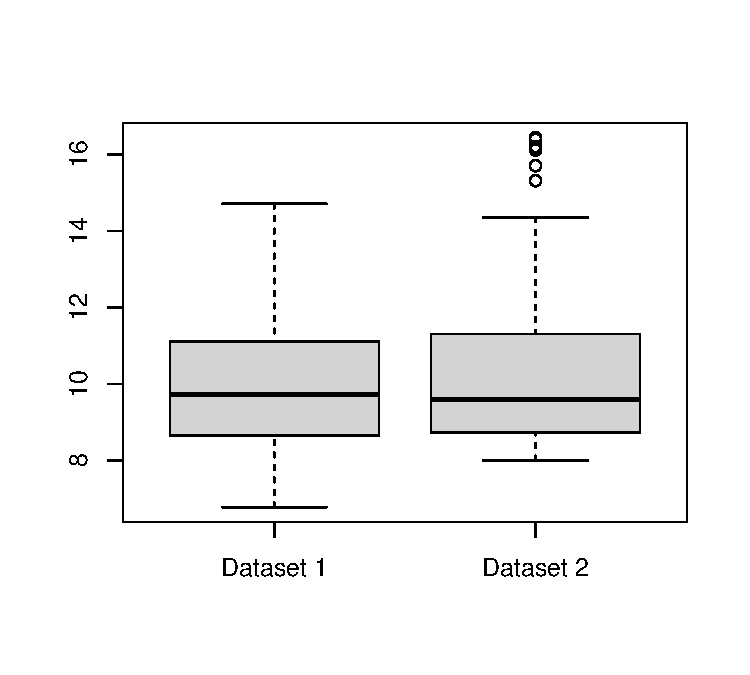
\includegraphics{math1710_files/figure-latex/unnamed-chunk-17-1.pdf}

\begin{myanswers}
\emph{Solution.} Some answers could be:

\begin{itemize}
\tightlist
\item
  The median and inter-quartile range of Dataset 2 appear to be very slightly larger than those in Dataset 1, although the differences are very small and might not be important in real life.
\item
  Dataset 2 has a few outliers; Dataset 1 has none.
\item
  While Dataset 1 is fairly ``balanced'' either side of the median, Dataset 2 shows what statisticians call a ``positive skew'': the data above the median is much more spread out than the data below the median.
\end{itemize}

\textbf{Group feedback:}
You can probably think of other answers.

\end{myanswers}

\hypertarget{P1-long-solutions}{%
\subsection*{B: Long questions}\label{P1-long-solutions}}
\addcontentsline{toc}{subsection}{B: Long questions}

\textbf{B1.} For each of the two datasets below, calculate the following summary statistics, or explain why it is not possible to do so: mode; median; mean; number of distinct outcomes; inter-quartile range; and sample variance.

\textbf{(a)} Shirt sizes for the \(n = 16\) members of a university football squad:

\begin{longtable}[]{@{}
  >{\centering\arraybackslash}p{(\columnwidth - 10\tabcolsep) * \real{0.3333}}
  >{\centering\arraybackslash}p{(\columnwidth - 10\tabcolsep) * \real{0.1667}}
  >{\centering\arraybackslash}p{(\columnwidth - 10\tabcolsep) * \real{0.1111}}
  >{\centering\arraybackslash}p{(\columnwidth - 10\tabcolsep) * \real{0.1111}}
  >{\centering\arraybackslash}p{(\columnwidth - 10\tabcolsep) * \real{0.1111}}
  >{\centering\arraybackslash}p{(\columnwidth - 10\tabcolsep) * \real{0.1667}}@{}}
\toprule\noalign{}
\begin{minipage}[b]{\linewidth}\centering
\textbf{Colour}
\end{minipage} & \begin{minipage}[b]{\linewidth}\centering
Xtra Small
\end{minipage} & \begin{minipage}[b]{\linewidth}\centering
Small
\end{minipage} & \begin{minipage}[b]{\linewidth}\centering
Medium
\end{minipage} & \begin{minipage}[b]{\linewidth}\centering
Large
\end{minipage} & \begin{minipage}[b]{\linewidth}\centering
Xtra Large
\end{minipage} \\
\midrule\noalign{}
\endhead
\bottomrule\noalign{}
\endlastfoot
\textbf{Number of shirts} & 0 & 1 & 6 & 4 & 5 \\
\end{longtable}

\begin{myanswers}
\emph{Solution.}
The modal shirt size is medium. The number of distinct outcomes is 4 (we don't quite ``Xtra Small'', which was not observed in the data).

This time, we can order the data from smallest to largest, even though the data is not numerical. Since \((16 + 1)/2 - 8.5\), the median datapoint is the 8th or 9th datapoints, which are Large.

Since \(1 + 0.25(16 - 1) = 4.75\) the lower quartile is the 4th or 5th datapoints, which are Medium. Since \(1 + 0.75(16-1) = 12.25\), the upper quartile is the 12th or 13th datapoints, which are Xtra Large. So we can certainly say that the inner quartiles range from Medium to Xtra Large. We could probably also say that the interquartile range is 3 shirt sizes (Medium, Large, Xtra Large).

Again, because the data is not numerical, we can't add it up, so can't calculate a mean or sample variance.

\end{myanswers}

\textbf{(b)} Six packets of Skittles are opened together, a total of \(n = 361\) sweets. The colours of these sweets is recorded as follows:

\begin{longtable}[]{@{}cccccc@{}}
\toprule\noalign{}
\textbf{Colour} & Red & Orange & Yellow & Green & Purple \\
\midrule\noalign{}
\endhead
\bottomrule\noalign{}
\endlastfoot
\textbf{Number of Skittles} & 67 & 71 & 87 & 74 & 62 \\
\end{longtable}

\begin{myanswers}
\emph{Solution.}
The modal colour is Yellow. The number of distinct outcomes is 5.

It's not possible to calculate the median or the quartiles, because, unlike numerical data, the colours can't be put ``in order'' from smallest to largest.

It's not possible to calculate the mean or sample variance, as these require us to have numerical data that can be ``added up'', but this can't be done with colours.

\textbf{Group feedback:} Make sure your explanation is clear for why we can't calculate a median for the Skittles data but can for the shirts: the key is whether or not the data can be \emph{ordered}.

\end{myanswers}

\textbf{B2.} A summary statistic is informally said to be ``robust'' if it typically doesn't change much if a small number of outliers are introduced to a large dataset, or ``sensitive'' if it often changes a lot when a small number of outliers are introduced. Briefly discuss the robustness or sensitivity of the following summary statistics: \textbf{(a)} mode; \textbf{(b)} median; \textbf{(c)} mean; \textbf{(d)} number of distinct outcomes; \textbf{(e)} inter-quartile range; and \textbf{(f)} sample variance.

\begin{myanswers}
\emph{Solutions.}

\textbf{(a)} An outlier will typically be the only data point with its value, or certainly rare. Therefore, the mode will typically not change at all if a small number of outliers are introduced, so is robust. (The exception is for data where every observation is likely to be different, so any outliers become ``joint modes'' along with everything else; but in this case the mode is not a useful statistic in the first place.)

\textbf{(b)} The introduction of outliers will typically only change the median a little bit, by shifting it between different nearby values in the ``central mass'' of the data. In particular, the \emph{size} of the outliers won't make any difference at all (only whether they are ``high outliers'' above the median or ``low outliers'' below the median). So the median is robust.

\textbf{(c)} The mean can change a lot if outliers are introduced, especially if the outlier is enormously far our from the data. So the mean is sensitive.

\textbf{(d)} The number of distinct outcomes will only increase by (at most) 1 for each outlier introduced. This is not typically a relevant increase, so the number of distinct outcomes is robust.

\textbf{(e)} The interquartile range is robust, for the same reason as the median.

\textbf{(f)} The sample variance is sensitive, for the same reason as the mean.

(You might like to think about situations where it's better to use a robust statistic or better to use a sensitive statistic.)

\textbf{Group feedback:} I find it helpful to suppose I was studying the net worth of people in my tutorial group, and calculating summary statistics. How would those statistics changed change if Elon Musk (owner of Tesla and Twitter, net worth roughly \$200 billion) joined my tutorial group? The mean and sample variance would change an enormous amount, while the median and interquartile range would barely change at all in comparison.

Remember that ``robust'' and ``sensitive'' are general descriptions rather than precise mathematical definitions. So it doesn't matter if you disagree with my opinions provided that you give clear and detailed explanations to back up your opinion.

\end{myanswers}

\textbf{B3.} Let \(\mathbf a = (a_1, a_2, \dots a_n)\) and \(\mathbf b = (b_1, b_2, \dots, b_n)\) be two real-valued vectors of the same length. Then the \emph{Cauchy--Schwarz inequality} says that
\[ \left( \sum_{i=1}^n a_i b_i \right)^2 \leq \left( \sum_{i=1}^n a_i^2 \right) \left(\sum_{i=1}^n b_i^2 \right) . \]

\textbf{(a)} By making a clever choice of \((a_i)\) and \((b_i)\) in the Cauchy--Schwarz inequality, show that \(s_{xy}^2 \leq s_x^2 s_y^2\).

\begin{myanswers}
\emph{Solutions.}
Recalling the formulas for \(s_{xy}\), \(s_x^2\), and \(s_y^2\),
\begin{align*}
s_{xy} &= \frac{1}{n-1} \sum_{i=1}^n (x_i - \bar x)(y_i - \bar y) ,\\
s_{x}^2 &= \frac{1}{n-1} \sum_{i=1}^n (x_i - \bar x)^2 ,\\
s_{y}^2 &= \frac{1}{n-1} \sum_{i=1}^n (y_i - \bar y)^2 ,
\end{align*}
and comparing them with the Cauchy--Schwarz inequality, it looks like taking \(a_i = x_i - \bar x\) and \(b_i = y_i - \bar y\) might be useful.

Making that substitution, we get
\[ \left( \sum_{i=1}^n (x_i - \bar x)(y_i - \bar y) \right)^2 \leq \left( \sum_{i=1}^n (x_i - \bar x)^2 \right) \left(\sum_{i=1}^n (y_i - \bar y)^2 \right) . \]

These are very close to the formulas for \(s_{xy}\), \(s_x^2\), and \(s_y^2\), but are just missing the ``\(1/(n-1)\)''s; what we in fact have is
\[ \left( (n-1) s_{xy} \right)^2 \leq (n-1)s_x^2 \cdot (n-1) s_y^2 .\]
Cancelling \((n-1)^2\) from each side, we have \(s_{xy}^2 \leq s_x^2 s_y^2\), as required.

\textbf{Group feedback:} Keep trying different choices for \((a_i)\) and \((b_i)\); maybe your first attempt won't work, but it pays to be persistent!

A fancier choice is \(a_i = (x_i - \bar x)/\sqrt{n-1}\) and \(b_i = (y_i - \bar y)/\sqrt{n-1}\), to get the exact result without needing a second cancellation step, but I would find that harder to spot.

\end{myanswers}

\textbf{(b)}
Hence, show that the correlation \(r_{xy}\) satisfies \(-1 \leq r_{xy} \leq 1\).

\begin{myanswers}
\emph{Solutions.}
Recall the formula for the correlation is
\[ r_{xy} = \frac{s_{xy}}{s_xs_y} . \]
We can make part (a) look a bit like this dividing both sides by \(s_x^2 s_y^2\), to get
\[\frac{s_{xy}^2}{s_x^2 s_y^2} \leq 1.   \]
In fact that's the square of the correlation on the left-hand side, so we've shown that \(r_{xy}^2 \leq 1\).

Finally, we note that if a number squared is less than or equal to 1, then the number must be between -1 and +1 inclusive. (Numbers bigger than 1 get bigger still when squared; numbers smaller than -1 become bigger than +1 when squared; numbers between -1 and +1 get closer to 0.) Hence we have shown that \(-1 \leq r_{xy} \leq 1\), as required.

\textbf{Group feedback:} In part (b) there's a temptation to ``square-root both sides of the inequality''. But you have to be extremely careful if you do this -- make sure you are properly accounting for the positive and negative square roots on both sides (if necessary), and where that does or doesn't require reversing the direction of the inequality. I recommend leaving the square-root operation until the last possible moment of the proof or, perhaps even better, reasoning through words as I did above.

Remember that you can still attempt part (b) even if you got stuck on part (a).

\end{myanswers}

\textbf{B4.} A researcher wishes to study the effect of mental health on academic achievement. The researcher will collect data on the mental health of a cohort of students by asking them to fill in a questionnaire, and will measure academic achievement via the students' scores on their university exams. Discuss some of the ethical issues associated with the collection, storage, and analysis of this data, and with the publication of the results of the analysis. Are there ways to mitigate these issues?

(It's not necessary to write an essay for this question -- a few short bulletpoints will suffice. There may be an opportunity to discuss these issues in more detail in your tutorial.)

\begin{myanswers}
\textbf{Group feedback:} There are no ``correct'' or ``incorrect'' answers here, but here are a few things that students in my own tutorials brought up, which may act as a prompt for your own discussions.

\begin{itemize}
\item
  It's important the students/subjects have given their consent for their data to be used this way. It must be ``informed consent'', where they understand for what purpose the data will be used, how it will be stored, and so on. It must be easy and painless for students to decline to take part.
\item
  Consideration should be given on how to anonymise the data as much as possible -- it's not necessary for those analysing the data to know which questionnaire or which exam result belongs to which student, only that the questionnaire and results can be paired up.
\item
  Even if after data is anonymised, care should be taken about whether the students could be worked out from the data. For example, if only one student did a certain combination of modules, their identity could ``leak'' that way. Perhaps imprecise data, such as classes rather than exact marks, might help maintain privacy while only slightly reducing the usefulness of the data?
\item
  On one hand, it seems like this data should perhaps be deleted once analysis has been carried out, for the privacy of the students. On the other hand, principles of ``open science'' suggest that the data should be kept -- and even publicly made available -- for other researchers to check the work. There are competing ethical considerations here.
\item
  If correlations are found in the data, care should be taken when publishing the analysis not to wrongly suggest a causation. (Just because X and Y are positively correlated, it doesn't mean that X \emph{causes} Y -- or that Y causes X.)
\end{itemize}

You can probably think of many other things.

\end{myanswers}

\end{document}
